\section{Interpolazione Polinomiale} 

\begin{exercise}[4.1] 
Trovare un polinomio $p(x)$ che interpola la funzione $f(x) = 4x^{2} -12x +1$
nei punti di ascissa $x_{i} = i$, con $ i \in \{ 0,\ldots, 4 \}$.
\end{exercise}
Per l'implementazione vedere il codice \nameref{subsec:exercise41} e per la 
sua esecuzione lanciare lo script \nameref{subsec:scriptForExercise41}.
\begin{center} 
% GNUPLOT: LaTeX picture with Postscript
\begingroup
  \makeatletter
  \providecommand\color[2][]{%
    \GenericError{(gnuplot) \space\space\space\@spaces}{%
      Package color not loaded in conjunction with
      terminal option `colourtext'%
    }{See the gnuplot documentation for explanation.%
    }{Either use 'blacktext' in gnuplot or load the package
      color.sty in LaTeX.}%
    \renewcommand\color[2][]{}%
  }%
  \providecommand\includegraphics[2][]{%
    \GenericError{(gnuplot) \space\space\space\@spaces}{%
      Package graphicx or graphics not loaded%
    }{See the gnuplot documentation for explanation.%
    }{The gnuplot epslatex terminal needs graphicx.sty or graphics.sty.}%
    \renewcommand\includegraphics[2][]{}%
  }%
  \providecommand\rotatebox[2]{#2}%
  \@ifundefined{ifGPcolor}{%
    \newif\ifGPcolor
    \GPcolortrue
  }{}%
  \@ifundefined{ifGPblacktext}{%
    \newif\ifGPblacktext
    \GPblacktexttrue
  }{}%
  % define a \g@addto@macro without @ in the name:
  \let\gplgaddtomacro\g@addto@macro
  % define empty templates for all commands taking text:
  \gdef\gplbacktext{}%
  \gdef\gplfronttext{}%
  \makeatother
  \ifGPblacktext
    % no textcolor at all
    \def\colorrgb#1{}%
    \def\colorgray#1{}%
  \else
    % gray or color?
    \ifGPcolor
      \def\colorrgb#1{\color[rgb]{#1}}%
      \def\colorgray#1{\color[gray]{#1}}%
      \expandafter\def\csname LTw\endcsname{\color{white}}%
      \expandafter\def\csname LTb\endcsname{\color{black}}%
      \expandafter\def\csname LTa\endcsname{\color{black}}%
      \expandafter\def\csname LT0\endcsname{\color[rgb]{1,0,0}}%
      \expandafter\def\csname LT1\endcsname{\color[rgb]{0,1,0}}%
      \expandafter\def\csname LT2\endcsname{\color[rgb]{0,0,1}}%
      \expandafter\def\csname LT3\endcsname{\color[rgb]{1,0,1}}%
      \expandafter\def\csname LT4\endcsname{\color[rgb]{0,1,1}}%
      \expandafter\def\csname LT5\endcsname{\color[rgb]{1,1,0}}%
      \expandafter\def\csname LT6\endcsname{\color[rgb]{0,0,0}}%
      \expandafter\def\csname LT7\endcsname{\color[rgb]{1,0.3,0}}%
      \expandafter\def\csname LT8\endcsname{\color[rgb]{0.5,0.5,0.5}}%
    \else
      % gray
      \def\colorrgb#1{\color{black}}%
      \def\colorgray#1{\color[gray]{#1}}%
      \expandafter\def\csname LTw\endcsname{\color{white}}%
      \expandafter\def\csname LTb\endcsname{\color{black}}%
      \expandafter\def\csname LTa\endcsname{\color{black}}%
      \expandafter\def\csname LT0\endcsname{\color{black}}%
      \expandafter\def\csname LT1\endcsname{\color{black}}%
      \expandafter\def\csname LT2\endcsname{\color{black}}%
      \expandafter\def\csname LT3\endcsname{\color{black}}%
      \expandafter\def\csname LT4\endcsname{\color{black}}%
      \expandafter\def\csname LT5\endcsname{\color{black}}%
      \expandafter\def\csname LT6\endcsname{\color{black}}%
      \expandafter\def\csname LT7\endcsname{\color{black}}%
      \expandafter\def\csname LT8\endcsname{\color{black}}%
    \fi
  \fi
  \setlength{\unitlength}{0.0500bp}%
  \begin{picture}(7680.00,5760.00)%
    \gplgaddtomacro\gplbacktext{%
      \colorrgb{0.00,0.00,0.00}%
      \put(866,634){\makebox(0,0)[r]{\strut{}-500}}%
      \colorrgb{0.00,0.00,0.00}%
      \put(866,1573){\makebox(0,0)[r]{\strut{}0}}%
      \colorrgb{0.00,0.00,0.00}%
      \put(866,2511){\makebox(0,0)[r]{\strut{}500}}%
      \colorrgb{0.00,0.00,0.00}%
      \put(866,3450){\makebox(0,0)[r]{\strut{}1000}}%
      \colorrgb{0.00,0.00,0.00}%
      \put(866,4388){\makebox(0,0)[r]{\strut{}1500}}%
      \colorrgb{0.00,0.00,0.00}%
      \put(866,5327){\makebox(0,0)[r]{\strut{}2000}}%
      \colorrgb{0.00,0.00,0.00}%
      \put(998,414){\makebox(0,0){\strut{}-20}}%
      \colorrgb{0.00,0.00,0.00}%
      \put(1742,414){\makebox(0,0){\strut{}-15}}%
      \colorrgb{0.00,0.00,0.00}%
      \put(2486,414){\makebox(0,0){\strut{}-10}}%
      \colorrgb{0.00,0.00,0.00}%
      \put(3230,414){\makebox(0,0){\strut{}-5}}%
      \colorrgb{0.00,0.00,0.00}%
      \put(3974,414){\makebox(0,0){\strut{}0}}%
      \colorrgb{0.00,0.00,0.00}%
      \put(4718,414){\makebox(0,0){\strut{}5}}%
      \colorrgb{0.00,0.00,0.00}%
      \put(5462,414){\makebox(0,0){\strut{}10}}%
      \colorrgb{0.00,0.00,0.00}%
      \put(6206,414){\makebox(0,0){\strut{}15}}%
      \colorrgb{0.00,0.00,0.00}%
      \put(6950,414){\makebox(0,0){\strut{}20}}%
    }%
    \gplgaddtomacro\gplfronttext{%
    }%
    \gplbacktext
    \put(0,0){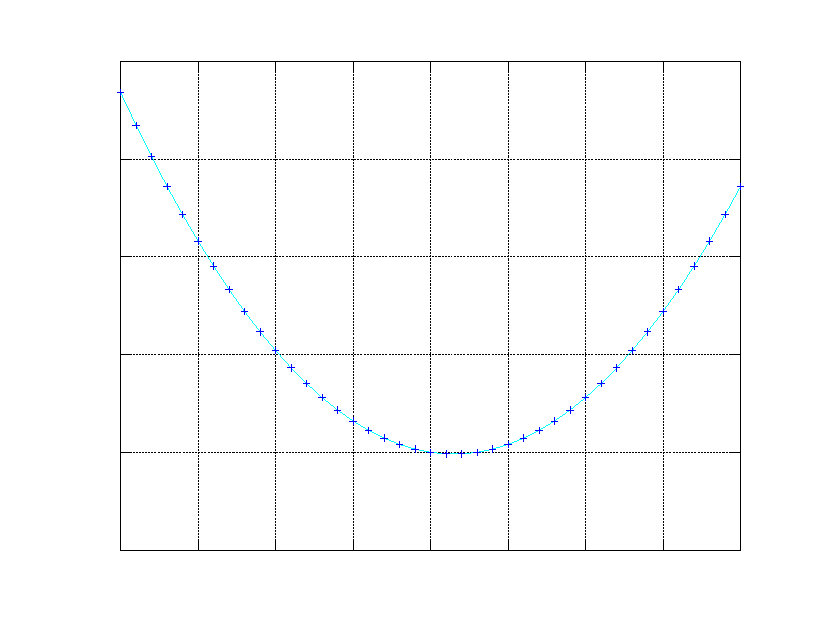
\includegraphics{ApprossimazioneFunzioni/exercise41PlotOutput}}%
    \gplfronttext
  \end{picture}%
\endgroup

\end{center}
In cyan \`e reppresentata la curva della funzione $f$, mentre con i simboli
$+$ sono rappresentati i punti interpolati dal polinomio $p$.

\begin{exercise}[4.2] 
Per il testo dell'esercizio consultare il libro di testo.
\end{exercise}
\begin{proof}
L'algoritmo riportato implementa questo schema (utilizzo gli indici nella
notazione usata nella formulazione matematica, quindi sono zero-based):
\begin{displaymath}
\begin{split}
	p^{(0)}(x) &= a_{n} \\
	p^{(i+1)}(x) &= p^{(i)}x + a_{n-i} 
\end{split}
\end{displaymath}
con $p^{(i)}$ indico il valore di $p$ all'$i$-esimo passo dei esecuzione. 
Se considero il valore di $p$ ad un generico passo $i$ di esecuzione si
osserva che ha questa struttura:
\begin{displaymath}
\begin{split}
	p^{(i)}(x) &= (a_{n}x^{i-1} + a_{n-1}x^{i-2} + \ldots + a_{n-i+1})x + a_{n-i}\\
	&= a_{n}x^{i} + a_{n-1}x^{i-1} + \ldots + a_{n-i+1}x + a_{n-i}
\end{split}
\end{displaymath}
Il polinomio $p^{(i)}$ \`e di grado $i$, quindi saturando l'indice $i$ arrivando
a calcolare $p^{n}$, si ottiene il polinomio:
\begin{displaymath}
	p(x) = p^{(n)}(x) = a_{n}x^{n} + a_{n-1}x^{n-1} + \ldots + a_{1}x + a_{0}
\end{displaymath}
Ovvero quello che si chiede nel problema.
\end{proof}

\begin{exercise}[4.3] 
Per il testo dell'esercizio consultare il libro di testo.
\end{exercise}
\begin{proof}
Dimostro i punti del \emph{Lemma 4.1}:
\begin{enumerate}
  \item \label{exercise43proofPoint1} questa \`e la forma di un generico
  polinomio $k$ della base di Lagrange di grado $n$:
  \begin{displaymath}
  L_{kn}(x) = \frac{(x-x_{0}) \cdots (x-x_{k-1})(x-x_{k+1})\cdots (x-x_{n})}
  	{(x_{k}-x_{0}) \cdots (x_{k}-x_{k-1})(x_{k}-x_{k+1})\cdots (x_{k}-x_{n})}
  \end{displaymath}
  Se valuto il polinomio $L_{kn}(x_{i})$ in una generica ascissa di
  interpolazione $x_{i}$ posso avere due casi:
  \begin{itemize}
    \item se $i \not = k$, allora $x_{i} \in \{
    x_{0},\ldots,x_{k-1},x_{k+1},\ldots,x_{n} \}$ ma questo fa si che uno dei
    fattori del numeratore abbia la forma $(x_{i} - x_{i}) = 0$ che annulla la
    produttoria:
    \begin{displaymath}
  L_{kn}(x_{i\not = k}) = \frac{(x_{i}-x_{0}) \cdots
  (x_{i}-x_{k-1})(x_{i}-x_{k+1})\cdots (x_{i}-x_{i}) \cdots (x_{i}-x_{n})}
  	{(x_{k}-x_{0}) \cdots (x_{k}-x_{k-1})(x_{k}-x_{k+1})\cdots (x_{k}-x_{n})} = 0
  \end{displaymath}
  Osservazione: ho inserito il termine che si annulla pi\`u a destra, ma il
  posizionamento \`e da ritenersi non influente in quanto per il prodotto
  l'ordine dei fattori non influisce ed inoltre \`e dipendente da $i$.
    \item se $i = k$ allora ottengo
    \begin{displaymath}
  L_{kn}(x_{i = k}) = \frac{(x_{k}-x_{0}) \cdots
  (x_{k}-x_{k-1})(x_{k}-x_{k+1})\cdots (x_{k}-x_{n})}
  	{(x_{k}-x_{0}) \cdots (x_{k}-x_{k-1})(x_{k}-x_{k+1})\cdots (x_{k}-x_{n})} = 1
  \end{displaymath}
  \end{itemize}
  
  \item i polinomi della base di Lagrange hanno grado esatto $n$ in quanto per
  definizione del generico polinomio $k$ si ha:
  \begin{displaymath}
  	L_{kn}(x) = \prod_{j=0 \quad j \not = k}^{n}{\frac{x-x_{j}}{x_{k}-x_{j}}}
  \end{displaymath}
  l'indice della produttoria ``corre'' da $0$ a $n$, indicizzando $n+1$
  posizioni, ma la $k$-esima posizione viene saltata, quindi vengono eseguiti
  $n$ prodotti, di conseguenza il termine di grado massimo \`e $x^{n}$.
  Inoltre posso dividera la produttoria in questo modo:
  \begin{displaymath}
  	L_{kn}(x) = \frac{\prod_{j=0; j \not =
  	k}^{n}{x-x_{j}}}{\prod_{j=0; j \not =
  	k}^{n}{x_{k}-x_{j}}}
  \end{displaymath}
  la quantit\`a al denominatore non dipende dall'ascissa $x$ in input, quindi si
  pu\`o sviluppare il prodotto al numeratore, ottenendo un polinomio di grado
  $n$, con coefficiente uguale a $1$, poi moltiplicare per la costante al
  denominatore, ottenendo il termine di grado massimo:
  \begin{displaymath}
  	a_{n}x^{n} = \frac{1}{\prod_{j=0; j \not = k}^{n}{x_{k}-x_{j}}} x^{n}
  \end{displaymath}
  
  \item per dimostrare che i polinomi $L_{kn}(x)$ formano una base per  
  $\prod_{n}$ allora devo dimostrare:
  \begin{displaymath}
  	\alpha_{0}L_{0n}(x)+ \ldots + \alpha_{n}L_{nn}(x) = 0 \Leftrightarrow
  	\alpha_{0} = \ldots = \alpha_{n} = 0 
  \end{displaymath}
  Il verso $\Leftarrow$ \`e ovvio. Per il verso $\Rightarrow$ invece valuto
  la combinazione lineare dei polinomi in una generica ascissa di
  interpolazione $x_{i}$ ottenendo:
  \begin{displaymath}
  	\alpha_{0}L_{0n}(x_{i})+ \ldots + \alpha_{n}L_{nn}(x_{i}) = 0  
  \end{displaymath}
  Per il punto \ref{exercise43proofPoint1} i termini $\alpha_{k}L_{kn}(x_{i}) =
  0$ se $i \not = k$, quindi rimane il solo elemento $\alpha_{i}L_{in}(x_{i})$. 
  Ma, sempre per il punto \ref{exercise43proofPoint1} vale $L_{in}(x_{i}) = 1$,
  quindi:
  \begin{displaymath}
  	0 = \alpha_{i}L_{in}(x_{i}) = \alpha_{i}  
  \end{displaymath}
  Ripetendo questo ragionamento per ogni ascissa di interpolazione si ottiene
  $\alpha_{0} = \ldots = \alpha_{n} = 0$ e il verso risulta dimostrato.
\end{enumerate}
\end{proof}

\begin{exercise}[4.4] 
Per il testo dell'esercizio consultare il libro di testo.
\end{exercise}
\begin{proof}
Dimostro i punti del \emph{Lemma 4.2}:
\begin{enumerate}
  \item	\label{exercise44ProofPoint1} 
  $w_{k+1}(x) = (x - x_{k})w_{k}(x) = (x - x_{k})(x - x_{k-1})w_{k-1}(x)
   = \ldots = (x - x_{k})\cdots (x - x_{0}) = \prod_{j = 0}^{k}{(x - x_{j})}$
   \item come si vede dal punto
   \ref{exercise44ProofPoint1}, valutare $w_{k}(x)$ richiede eseguire $k$
   prodotti, per cui si ottiene un polinomio di grado $k$, quindi $w_{k}(x) \in
   \prod_{k}$
   \item valutare il polinomio $w_{k}$ in una delle ascisse di interpolazione
   $x_{i}$ con $i<k$, ovvero $w_{k}(x_{i})$ si ha che uno dei fattori di
   $w_{k}(x_{i}) = (x_{i} - x_{k-1})\cdots (x_{i} - x_{i}) \cdots (x_{i} -
   x_{0})$ si annulli, annullando di conseguenza tutta la produttoria, quindi
   vale $i<k \Rightarrow w_{k}(x_{i}) = 0 $.
   \item per dimostrare che i polinomi $w_{k}(x)$ formano una base per  
  $\prod_{k}$ allora devo dimostrare:
  \begin{displaymath}
  	\alpha_{0}w_{0}(x)+ \ldots + \alpha_{k}w_{k}(x) = 0 \Leftrightarrow
  	\alpha_{0} = \ldots = \alpha_{k} = 0 
  \end{displaymath}
  Sviluppo per chiarezza la precedente combinazione lineare:
  \begin{displaymath}
  	\alpha_{0} + \alpha_{1}(x - x_{0}) + \alpha_{2}(x - x_{1})(x - x_{0}) \ldots
  	+ \alpha_{k}(x - x_{k-1})\cdots(x - x_{0}) = 0
  \end{displaymath}
  Il verso $\Leftarrow$ \`e ovvio. Per il verso $\Rightarrow$ invece valuto
  la combinazione lineare dei polinomi in una generica ascissa di
  interpolazione $x_{i} \in \{ x_{0}, \ldots, x_{k} \}$ ottenendo:
  \begin{displaymath}
  	\alpha_{0}w_{0}(x_{i})+ \ldots + \alpha_{k}w_{k}(x_{i}) = 0   
  \end{displaymath}
  Posso ragionare distinguendo due casi:
  \begin{itemize}
    \item se $i = k$ allora $\forall j \in \{ 0, k \}:w_{j}(x_{i}) \not = 0$, in
    quanto per ipotesi le ascisse di interpolazione sono tutte distinte. 
    Per ipotesi di questo verso, la combinazione lineare degli elementi della
    base deve annullarsi, quindi affinche l'ipotesi venga rispettata deve valere 
    $\alpha_{0} = \ldots = \alpha_{k} = 0$
    \item se $i < k$ allora tutti i termini della forma $w_{j}(x_{i}) = 0$ se
    $i < j$. Possono per\`o rimanere dei termini per cui  $w_{r}(x_{i}) \not =
    0$ se $i \geq r$. Ma per questi termini posso ragionare come fatto nel caso
    di $i < k$, ottenendo che $\alpha_{0} = \ldots = \alpha_{r} = 0$.
  \end{itemize}
   Ripetendo questo ragionamento per ogni ascissa di interpolazione si ottiene
  $\alpha_{0} = \ldots = \alpha_{k} = 0$ e il verso risulta dimostrato.
 \end{enumerate}
\end{proof}

\begin{exercise}[4.5] 
Per il testo dell'esercizio consultare il libro di testo.
\end{exercise}
\begin{proof} Dimostro i punti del teorema in ordine di come vengono richiesti
dall'\emph{esercizio 4.5}:
\begin{enumerate}
  \item chiamo $w(x) = \alpha f(x) + \beta g(x)$, posso riscrivere:
  \begin{displaymath}
  \begin{split}
  	w(x)[x_{0}, \ldots, x_{r}] &= \sum_{j = 0}^{r}{
  		\frac{w(x_{j})}{\prod_{l = 0;l \not = j}^{r}{(x_{j} - x_{l})}}} = 
  		\sum_{j = 0}^{r}{
  		\frac{\alpha f(x_{j}) + \beta g(x_{j})}{\prod_{l = 0;l \not = j}^{r}{(x_{j}
  		- x_{l})}}} =\\
  	&= \sum_{j = 0}^{r}{
  		\frac{\alpha f(x_{j})}{\prod_{l = 0;l \not = j}^{r}{(x_{j} - x_{l})}}} +
  		\sum_{j = 0}^{r}{
  		\frac{\beta g(x_{j})}{\prod_{l = 0;l \not = j}^{r}{(x_{j} - x_{l})}}} = \\
  	&=	\alpha \sum_{j = 0}^{r}{
  		\frac{ f(x_{j})}{\prod_{l = 0;l \not = j}^{r}{(x_{j} - x_{l})}}} +
  		\beta \sum_{j = 0}^{r}{
  		\frac{ g(x_{j})}{\prod_{l = 0;l \not = j}^{r}{(x_{j} - x_{l})}}} = \\
  	&=	\alpha f(x)[x_{0}, \ldots, x_{r}] + \beta g(x)[x_{0}, \ldots, x_{r}]
  \end{split}
  \end{displaymath}
  
  \item esiste una matrice di permutazione $P \in \mathbb{R}^{(r+1) \times
  (r+1)}$ tale che permette di costruire un vettore $\vect{i}$:
  \begin{displaymath}
  	\vect{i} = \begin{bmatrix}
  		i_{0} \\ 
  		\vdots \\
  		i_{r}
  	\end{bmatrix} = P\begin{bmatrix}
  		0 \\ 
  		\vdots \\
  		r
  	\end{bmatrix}
  \end{displaymath}
  in modo, usando la simmetria dell'operatore $\sum$ e dell'operatore $\prod$, 
  da verificare $f(x)[x_{0}, \ldots, x_{r}] = f(x)[x_{i_{0}}, \ldots,
  x_{i_{r}}]$
  
  \item sia $f \in \prod_{k}$ la funzione da approssimare e si assuma che
  questa sia definita con il seguente polinomio:
  \begin{displaymath}
  	f(x) = \sum_{i = 0}^{k}{a_{k}x^{k}}
  \end{displaymath}
  Analizzo $f[x_{0}, \ldots, x_{r}]$ distinguendo due casi:
  \begin{itemize}
    \item se $k = r$ allora 
    \begin{displaymath}
    	f[x_{0}, \ldots, x_{r}] = f[x_{0}, \ldots, x_{k}] = 
    	\sum_{j = 0}^{k}{
  		\frac{f_{j}}{\prod_{l = 0;l \not = j}^{k}{(x_{j} - x_{l})}}}
    \end{displaymath}
    Sia $p_{r}\in \prod_{r}$ il polinomio interpolante la funzione
    $f$. Per ipotesi del problema, $f$ \`e un polinomio e stiamo analizzando
    per $k = r$, quindi $p_{k = r}$ e $f$ hanno lo stesso grado. Inoltre, per
    l'unicit\`a del polinomio interpolante, \`e vero che i coefficienti dei
    termini $x^{i}$ devono coincidere, di conseguenza vale quanto detto anche
    per il termine principale:
    \begin{displaymath}
    	f[x_{0}, \ldots, x_{k}] x^{k} = 
    	%\sum_{j = 0}^{k}{
  		%\frac{f_{j}}{\prod_{l = 0;l \not = j}^{k}{(x_{j} - x_{l})}}} x^{k} = 
  		a_{k}x^{k} \Rightarrow f[x_{0}, \ldots, x_{k}] = a_{k} 
    \end{displaymath}
    
    \item se $k < r$: 
    sia $p_{r}\in \prod_{r}$ il polinomio interpolante la funzione $f$.
    Per ipotesi del problema, $f$ \`e un polinomio e stiamo analizzando
    per $k < r$, quindi $p_{r}$ ha un grado maggiore di $f$. 
    Per l'unicit\`a del polinomio interpolante, essendo $f$ un
    polinomio (interpolante se stesso), allora $p_{r}$ deve coincidere con il 
    polinomio $f$. Per definizione, $p_{r}$ ha questa forma:
    \begin{displaymath}
    	p_{r}(x) = \sum_{j = 0}^{r}{f[x_{0}, \ldots, x_{j}] \omega_{j}(x)}
    \end{displaymath}
    ma tutti i termini $f[x_{0}, \ldots, x_{i}] \omega_{i}(x) = 0, k < i \leq r$
    devono annullarsi in ordine di avere $p_{k}$ coincidente con $f$. Affinch\`e
    si annullino \`e strettamente necessario che si annulli $f[x_{0}, \ldots,
    x_{i}] = 0$ in quanto $\omega_{i} \in \prod_{r}$ non pu\`o annullarsi
    perch\`e \`e un vettore della base di $\prod_{r}$. Se fosse vero che
    $\omega_{i}(x) = 0$ allora si produrrebbe un assurdo in quanto per ipotesi 
    $p_{k} \in \prod_{r}$ ma questo spazio non sarebbe di grado $r$ (ma di grado
    pi\`u basso).
  \end{itemize}
  
  \item devo dimostrare che se $f \in \mathcal{C}^{(r)}$ allora $\exists \xi
  \in [\min_{i}\{x_{i}\}, \ldots, \max_{i}\{x_{i}\}]$ tale che:
  \begin{displaymath}
  	f[x_{0}, \ldots, x_{r}] = \frac{f^{(r)}(\xi)}{r!}
  \end{displaymath}
  
  Sia $p_{r} \in \prod_{r}$ il polinomio interpolante, chiamo $e(x) = f(x) -
  p_{r}(x)$, con $e \in \mathcal{C}^{(r)}$. Si osserva che per costruzione del
  polinomio $e$, vale $e(x_{i}) = 0, \forall x_{i} \in \{x_{0}, \ldots, x_{r}\}$
  insieme delle ascisse di interpolazione.
  
  Per il teorema di Rolle $\exists \xi_{0}^{(1)}: e'(\xi_{0}^{(1)}) = 0$.
  Astraendo ottengo:
  \begin{displaymath}
 	x_{0} < \xi_{0}^{(1)} < x_{1} < \xi_{1}^{(1)} < x_{2} < \ldots < x_{r-1} <
 	\xi_{r-1}^{(1)} < x_{r} \quad \wedge \quad \forall i \in \{ 0, \ldots, r-1\}:
 	e'(\xi_{i}^{(1)}) = 0
  \end{displaymath}
  % questo implica che e ha punti di massimo o minimo in \xi_{i}^{(1)}
  Posso derivare $r$ volte perch\`e $e \in \mathcal{C}^{(r)}$ ottenendo:
  \begin{displaymath}
  \begin{split}
 	\forall i \in \{ 0, \ldots, r-1\}&:	e^{(1)}(\xi_{i}^{(1)}) = 0 \\
 	\forall i \in \{ 0, \ldots, r-1\}&:	e^{(2)}(\xi_{i}^{(2)}) = 0 \\
 	& \vdots \\
 	\forall i \in \{ 0, \ldots, r-1\}&:	e^{(r)}(\xi_{i}^{(r)}) = 0
  \end{split}
  \end{displaymath}
  Posso astrarre sui $\xi_{i}^{(k)}$ sia sull'indice $i$ della posizione, sia
  sull'indice $k$ dell'ordine della derivata (in quanto in tutti la derivata
  $r$-esima di $e$ si annulla) e considerare un generico $\xi$.
  
  Derivo $r$ volte l'equazione $e(x) = f(x) - p_{r}(x)$ ottenendo 
  $e^{(r)}(x) = f^{(r)}(x) -  p_{r}^{(r)}(x)$ e valuto in $\xi$:
  \begin{displaymath}
  	0 = e^{(r)}(\xi) = f^{(r)}(\xi) -  p_{r}^{(r)}(\xi)
  \end{displaymath}
  Per definizione $p_{r}$ ha questa struttura:
  \begin{displaymath}
  	p_{r}(x) = f[x_{0}] \omega_{0}(x) + f[x_{0}, x_{1}] \omega_{1}(x) + \ldots + 
  		f[x_{0}, \ldots, x_{k}]\omega_{k}(x) + \ldots + 
  		f[x_{0}, \ldots, x_{r}]\omega_{r}(x) \quad, k < r
  \end{displaymath}
  Se derivo $r$ volte, ottengo che i termini $f[x_{0}, \ldots,
  x_{k}]\omega_{k}^{(r)}(x)$ con $k < r$ si annullano per definizione
  dell'operatore derivata. Rimane solo il termine $f[x_{0}, \ldots,
  x_{r}]\omega_{r}(x)$. Ma anche per questo termine possiamo applicare lo stesso
  ragionamento, ovvero se si considera i termini generati da 
  $\omega_{r}(x) = x^{r} + \alpha_{r-1}x^{r-1} + \ldots + \alpha_{1}x +
  \alpha_{0}$, quando si deriva $r$ volte si ottiene: 
  \begin{displaymath}
  \begin{split}
  	\omega_{r}^{(r)} = \frac{\vartheta^{(r)}(x^{r})}{\vartheta x} + 
  		\frac{\vartheta^{(r)}(\alpha_{r-1}x^{r-1})}{\vartheta x} + \ldots &+ 
  		\frac{\vartheta^{(r)}(\alpha_{i}x^{i})}{\vartheta x} + \ldots +
  		\frac{\vartheta^{(r)}(\alpha_{1}x)}{\vartheta x} + 
  		\frac{\vartheta^{(r)}(\alpha_{0})}{\vartheta x} = 
  		\frac{\vartheta^{(r)}(x^{r})}{\vartheta x} = r! \\
  	\text{con } i < r &\Rightarrow
  	\frac{\vartheta^{(r)}(\alpha_{i}x^{i})}{\vartheta x} = 0
  \end{split}
  \end{displaymath}
  Quindi rimane l'unico termine $\alpha_{r} x^{r}$, che derivato $r$ volte
  produce $\frac{\vartheta^{(r)}(x^{r})}{\vartheta x} = r!$. Osservazione: dato
  che $\omega_{r}$ produce un polinomio monico, e si considera solo il termine
  principale, allora $\alpha_{r} = 1$. Riassumendo:
  \begin{displaymath}
  \begin{split}
  	0 = f^{(r)}(\xi) -  p_{r}^{(r)}(\xi) &= f^{(r)}(\xi) - 
  	f[x_{0}, \ldots, x_{r}] r! \\
  	f[x_{0}, \ldots, x_{r}] &= \frac{f^{(r)}(\xi)}{r!}
  \end{split}
  \end{displaymath}
  
  \item Prova per induzione su $r$.
  \begin{itemize}
    \item \emph{Base}:
    \begin{displaymath}
    	f[x_{0}, x_{1}] = \frac{f_{0}}{x_{0} - x_{1}} + \frac{f_{1}}{x_{1} - x_{0}}
    	= \frac{f_{1} - f_{0}}{x_{1} - x_{0}} = \frac{f[x_{1}] - f[x_{0}]}{x_{1} -
    	x_{0}}
    \end{displaymath}
  
  \item \emph{Induction hypothesis}: suppongo vero l'asserto per $r$ e dimostro
  per $r+1$
  \item \emph{Induction step}: devo far vedere che vale la seguente:
  	\begin{equation}
  	\label{eq:inductionStepExer45}
    	f[x_{0},\ldots, x_{r+1}] = 
    	\frac{ f[x_{1},\ldots, x_{r+1}] - f[x_{0},\ldots, x_{r}]}{x_{r+1} - x_{0}}
    \end{equation}
    Studio i termini che compaiono al numeratore:
    \begin{displaymath}
    	\sum_{j = 1}^{r+1}{
  		\frac{f_{j}}{\prod_{l = 1;l \not = j}^{r+1}{(x_{j} - x_{l})}}} - 
  		\sum_{j = 0}^{r}{
  		\frac{f_{j}}{\prod_{l = 0;l \not = j}^{r}{(x_{j} - x_{l})}}} = 
  	\end{displaymath}
  	Metto in evidenza la sommatoria, con indice $j \in \{1,\ldots,r\} = J$;
  	l'insieme $J$ \`e l'intersezione degli insiemi sui cui ``corrono''
  	entrambi gli indici delle due sommatorie che sto fattorizzando:
  	\begin{equation}
  	\label{eq:tripleAddendSumExer45}
     	= \sum_{j = 1}^{r}{
  		f_{j} \left ( \frac{1}{\prod_{l = 1;l \not = j}^{r+1}{(x_{j} - x_{l})}} -
  		\frac{1}{\prod_{l = 0;l \not = j}^{r}{(x_{j} - x_{l})}}
  		\right)} + 
  		% non posso lasciare 
  		% \frac{1}{\prod_{l = 1;l \not = j}^{r+1}{(x_{j} - x_{l})}} in quanto 
  		% l'indice j non sarebbe definito
  		\frac{f_{r+1}}{\prod_{l = 1}^{r}{(x_{r+1} - x_{l})}} -
  		\frac{f_{0}}{\prod_{l = 1}^{r}{(x_{0} - x_{l})}}
  	\end{equation}
  	Studio il primo addendo della \ref{eq:tripleAddendSumExer45}:
  	\begin{displaymath}
  	\begin{split}
     	& \sum_{j = 1}^{r}{
  		f_{j} \left ( \frac{1}{\prod_{l = 1;l \not = j}^{r+1}{(x_{j} - x_{l})}} -
  		\frac{1}{\prod_{l = 0;l \not = j}^{r}{(x_{j} - x_{l})}}
  		\right)} = 
  		\sum_{j = 1}^{r}{
  		\frac{f_{j}}{\prod_{l = 1;l \not = j}^{r}{(x_{j} - x_{l})}} 
  		\left (
  		\frac{1}{x_{j} - x_{r+1}} -
  		\frac{1}{x_{j} - x_{0}}
  		\right)} \\
  		&= \sum_{j = 1}^{r}{
  		\frac{f_{j}}{\prod_{l = 1;l \not = j}^{r}{(x_{j} - x_{l})}} 
  		\left (
  		\frac{(x_{j} - x_{0})-(x_{j} - x_{r+1})}{(x_{j} - x_{r+1})(x_{j} - x_{0})}
  		\right)} = 
  		\sum_{j = 1}^{r}{
  		\frac{f_{j}(x_{r+1} - x_{0})}{\prod_{l = 0;l \not = j}^{r+1}{(x_{j} -
  		x_{l})}}}
  	\end{split}
  	\end{displaymath}
  	Come si nota nella \ref{eq:inductionStepExer45}, 
  	questa quantit\`a deve essere raggruppata per $x_{r+1} - x_{0}$, quindi:
  	\begin{displaymath}
  	\begin{split} 
  		\sum_{j = 1}^{r}{
  		\frac{f_{j}(x_{r+1} - x_{0})}{\prod_{l = 0;l \not = j}^{r+1}{(x_{j} -
  		x_{l})}}} \left(\frac{1}{x_{r+1} - x_{0}}\right ) = 
  		\sum_{j = 1}^{r}{
  		\frac{f_{j}}{\prod_{l = 0;l \not = j}^{r+1}{(x_{j} -
  		x_{l})}}}
  	\end{split}
  	\end{displaymath}
  	Componendo questi passi si ottiene:
  	\begin{equation}
  	\label{eq:firstIntermediateResultExer45}
  	\begin{split} 
  		\sum_{j = 1}^{r}{
  		f_{j} \left ( \frac{1}{\prod_{l = 1;l \not = j}^{r+1}{(x_{j} - x_{l})}} -
  		\frac{1}{\prod_{l = 0;l \not = j}^{r}{(x_{j} - x_{l})}}
  		\right)} \left(\frac{1}{x_{r+1} - x_{0}}\right) = 
  		\sum_{j = 1}^{r}{
  		\frac{f_{j}}{\prod_{l = 0;l \not = j}^{r+1}{(x_{j} -
  		x_{l})}}}
  	\end{split}
  	\end{equation}
  	Studio il secondo addendo della \ref{eq:tripleAddendSumExer45} applicando il
  	raggruppamento $x_{r+1} - x_{0}$ come primo passo; come secondo passo
  	``sincronizzo'' l'indice della produttoria per essere ``compatibile'' 
  	con l'indice della produttoria che appare nel denomitore della
  	\ref{eq:firstIntermediateResultExer45}:
  	\begin{displaymath}
  	\frac{f_{r+1}}{\prod_{l = 1}^{r}{(x_{r+1} - x_{l})}}  \left(\frac{1}{x_{r+1}
  	- x_{0}}\right) = \frac{f_{r+1}}{\prod_{l = 0}^{r}{(x_{r+1} - x_{l})}} = 
  	\frac{f_{r+1}}{\prod_{l = 0;l \not = r+1}^{r+1}{(x_{r+1} - x_{l})}}
  	\end{displaymath}
  	Ho ottenuto il $(r+1)$-esimo termine della sommatoria principale, quindi
  	sommo questo risultato alla \ref{eq:firstIntermediateResultExer45}:
  	\begin{equation}
  	\label{eq:secondIntermediateResultExer45}
  	\sum_{j = 1}^{r}{
  		\frac{f_{j}}{\prod_{l = 0;l \not = j}^{r+1}{(x_{j} -
  		x_{l})}}} + 
  	\frac{f_{r+1}}{\prod_{l = 0;l \not = r+1}^{r+1}{(x_{r+1} - x_{l})}} =
  	\sum_{j = 1}^{r+1}{
  		\frac{f_{j}}{\prod_{l = 0;l \not = j}^{r+1}{(x_{j} -
  		x_{l})}}} 
  	\end{equation}
  	
  	Studio il terzo addendo della \ref{eq:tripleAddendSumExer45} applicando il
  	raggruppamento $x_{r+1} - x_{0}$: 
  	\begin{displaymath}
  	\frac{f_{0}}{\prod_{l = 1}^{r}{(x_{0} - x_{l})}}  \left(\frac{1}{x_{r+1}
  	- x_{0}}\right)
  	\end{displaymath}
  	e sommo algebricamente alla \ref{eq:secondIntermediateResultExer45}:
  	\begin{displaymath}
  	\begin{split}
	  	\sum_{j = 1}^{r+1}{
	  		\frac{f_{j}}{\prod_{l = 0;l \not = j}^{r+1}{(x_{j} -
	  		x_{l})}}} -
	  	\frac{f_{0}}{\prod_{l = 1}^{r}{(x_{0} - x_{l})}}  \left(\frac{1}{x_{r+1}
	  	- x_{0}}\right) =	  	\\
	  	= \sum_{j = 1}^{r+1}{
	  		\frac{f_{j}}{\prod_{l = 0;l \not = j}^{r+1}{(x_{j} -
	  		x_{l})}}} +
	  	\frac{f_{0}}{\prod_{l = 1}^{r}{(x_{0} - x_{l})}}  \left(\frac{1}{x_{0}
	  	- x_{r+1}}\right) = 
  	\end{split}
  	\end{displaymath}
  	``sincronizzo'' l'indice della produttoria per essere ``compatibile'' 
  	con l'indice della produttoria che appare nel denomitore del primo termine:
  	\begin{displaymath}
	  	= \sum_{j = 1}^{r+1}{
	  		\frac{f_{j}}{\prod_{l = 0;l \not = j}^{r+1}{(x_{j} -
	  		x_{l})}}} +
	  	\frac{f_{0}}{\prod_{l = 0;l\not = 0}^{r+1}{(x_{0} - x_{l})}} = 
  	\end{displaymath}
  	Con il secondo termine ho ottenuto lo $(0)$-esimo termine della sommatoria
  	principale, quindi posso includerlo nella sommatoria principale
  	modificando il range su cui ``corre'' l'indice $j$:
  	\begin{equation}
  	\label{eq:thirdIntermediateResultExer45} 
  		= \sum_{j = 0}^{r+1}{
	  		\frac{f_{j}}{\prod_{l = 0;l \not = j}^{r+1}{(x_{j} -
	  		x_{l})}}} = f[x_{0}, \ldots, x_{r+1}]
	\end{equation}
  	questo completa il passo induttivo.
  \end{itemize}
\end{enumerate}
\end{proof}

\begin{exercise}[4.6]
Per il testo dell'esercizio consultare il libro di testo.
\end{exercise}
Vedi il codice \nameref{subsec:differenzeDiviseEngineCode}.

\begin{exercise}[4.7]
Per il testo dell'esercizio consultare il libro di testo.
\end{exercise}
Vedi il codice \nameref{subsec:HornerGeneralizzato}. Per generare i risultati
che sto per descrivere, lanciare la funzione definita in
\nameref{subsec:exercise47testing}.

Ho considerato la funzione:
\begin{displaymath}
 f(x) = \frac{1}{1 + x^{2}}
\end{displaymath}
fissando come ascisse di intepolazione $x \in linspace(-3, 3,30) = \mathcal{x}$,
con $linspace$ intendo la funzione di \emph{Octave}.

Il seguente grafico mostra l'interpolazione della funzione $f$ utilizzando
l'algoritmo di \emph{Horner generalizzato} (implementato in
\nameref{subsec:HornerGeneralizzato}) in ascisse $\hat{x} \in [-5:0.5:5],
[-5:1:5], [-5:2:5]$, corrispondenti rispettivamente alle curve cyan, verde,
rosso. In blu la funzione reale $f$.
\begin{center} 
% GNUPLOT: LaTeX picture with Postscript
\begingroup
  \makeatletter
  \providecommand\color[2][]{%
    \GenericError{(gnuplot) \space\space\space\@spaces}{%
      Package color not loaded in conjunction with
      terminal option `colourtext'%
    }{See the gnuplot documentation for explanation.%
    }{Either use 'blacktext' in gnuplot or load the package
      color.sty in LaTeX.}%
    \renewcommand\color[2][]{}%
  }%
  \providecommand\includegraphics[2][]{%
    \GenericError{(gnuplot) \space\space\space\@spaces}{%
      Package graphicx or graphics not loaded%
    }{See the gnuplot documentation for explanation.%
    }{The gnuplot epslatex terminal needs graphicx.sty or graphics.sty.}%
    \renewcommand\includegraphics[2][]{}%
  }%
  \providecommand\rotatebox[2]{#2}%
  \@ifundefined{ifGPcolor}{%
    \newif\ifGPcolor
    \GPcolortrue
  }{}%
  \@ifundefined{ifGPblacktext}{%
    \newif\ifGPblacktext
    \GPblacktexttrue
  }{}%
  % define a \g@addto@macro without @ in the name:
  \let\gplgaddtomacro\g@addto@macro
  % define empty templates for all commands taking text:
  \gdef\gplbacktext{}%
  \gdef\gplfronttext{}%
  \makeatother
  \ifGPblacktext
    % no textcolor at all
    \def\colorrgb#1{}%
    \def\colorgray#1{}%
  \else
    % gray or color?
    \ifGPcolor
      \def\colorrgb#1{\color[rgb]{#1}}%
      \def\colorgray#1{\color[gray]{#1}}%
      \expandafter\def\csname LTw\endcsname{\color{white}}%
      \expandafter\def\csname LTb\endcsname{\color{black}}%
      \expandafter\def\csname LTa\endcsname{\color{black}}%
      \expandafter\def\csname LT0\endcsname{\color[rgb]{1,0,0}}%
      \expandafter\def\csname LT1\endcsname{\color[rgb]{0,1,0}}%
      \expandafter\def\csname LT2\endcsname{\color[rgb]{0,0,1}}%
      \expandafter\def\csname LT3\endcsname{\color[rgb]{1,0,1}}%
      \expandafter\def\csname LT4\endcsname{\color[rgb]{0,1,1}}%
      \expandafter\def\csname LT5\endcsname{\color[rgb]{1,1,0}}%
      \expandafter\def\csname LT6\endcsname{\color[rgb]{0,0,0}}%
      \expandafter\def\csname LT7\endcsname{\color[rgb]{1,0.3,0}}%
      \expandafter\def\csname LT8\endcsname{\color[rgb]{0.5,0.5,0.5}}%
    \else
      % gray
      \def\colorrgb#1{\color{black}}%
      \def\colorgray#1{\color[gray]{#1}}%
      \expandafter\def\csname LTw\endcsname{\color{white}}%
      \expandafter\def\csname LTb\endcsname{\color{black}}%
      \expandafter\def\csname LTa\endcsname{\color{black}}%
      \expandafter\def\csname LT0\endcsname{\color{black}}%
      \expandafter\def\csname LT1\endcsname{\color{black}}%
      \expandafter\def\csname LT2\endcsname{\color{black}}%
      \expandafter\def\csname LT3\endcsname{\color{black}}%
      \expandafter\def\csname LT4\endcsname{\color{black}}%
      \expandafter\def\csname LT5\endcsname{\color{black}}%
      \expandafter\def\csname LT6\endcsname{\color{black}}%
      \expandafter\def\csname LT7\endcsname{\color{black}}%
      \expandafter\def\csname LT8\endcsname{\color{black}}%
    \fi
  \fi
  \setlength{\unitlength}{0.0500bp}%
  \begin{picture}(7680.00,5760.00)%
    \gplgaddtomacro\gplbacktext{%
      \colorrgb{0.00,0.00,0.00}%
      \put(866,634){\makebox(0,0)[r]{\strut{}0}}%
      \colorrgb{0.00,0.00,0.00}%
      \put(866,1573){\makebox(0,0)[r]{\strut{}0.2}}%
      \colorrgb{0.00,0.00,0.00}%
      \put(866,2511){\makebox(0,0)[r]{\strut{}0.4}}%
      \colorrgb{0.00,0.00,0.00}%
      \put(866,3450){\makebox(0,0)[r]{\strut{}0.6}}%
      \colorrgb{0.00,0.00,0.00}%
      \put(866,4388){\makebox(0,0)[r]{\strut{}0.8}}%
      \colorrgb{0.00,0.00,0.00}%
      \put(866,5327){\makebox(0,0)[r]{\strut{}1}}%
      \colorrgb{0.00,0.00,0.00}%
      \put(998,414){\makebox(0,0){\strut{}-3}}%
      \colorrgb{0.00,0.00,0.00}%
      \put(1990,414){\makebox(0,0){\strut{}-2}}%
      \colorrgb{0.00,0.00,0.00}%
      \put(2982,414){\makebox(0,0){\strut{}-1}}%
      \colorrgb{0.00,0.00,0.00}%
      \put(3974,414){\makebox(0,0){\strut{}0}}%
      \colorrgb{0.00,0.00,0.00}%
      \put(4966,414){\makebox(0,0){\strut{}1}}%
      \colorrgb{0.00,0.00,0.00}%
      \put(5958,414){\makebox(0,0){\strut{}2}}%
      \colorrgb{0.00,0.00,0.00}%
      \put(6950,414){\makebox(0,0){\strut{}3}}%
    }%
    \gplgaddtomacro\gplfronttext{%
    }%
    \gplbacktext
    \put(0,0){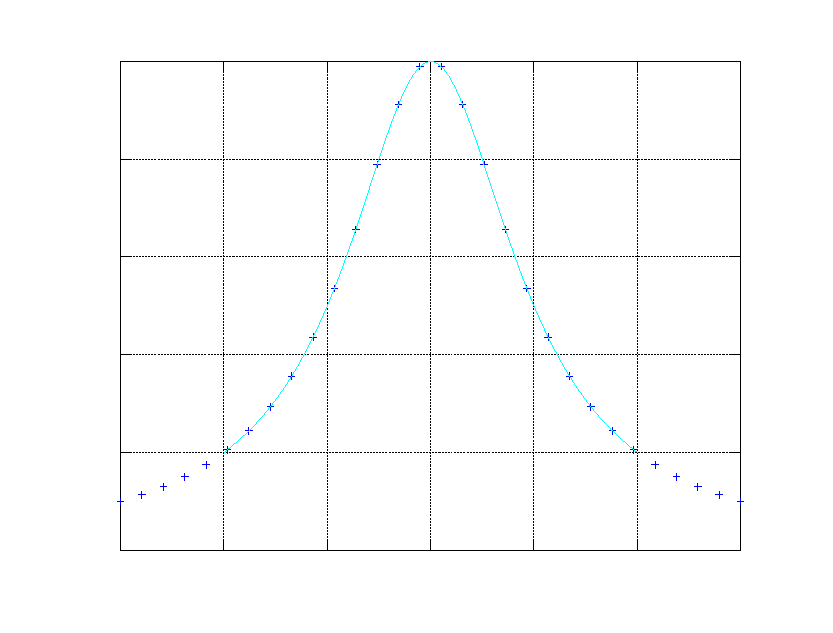
\includegraphics{ApprossimazioneFunzioni/exercise47-CorrectPlotOutput}}%
    \gplfronttext
  \end{picture}%
\endgroup

\end{center}

Dimostro che l'algoritmo  \nameref{subsec:HornerGeneralizzato} valuta il
polinomio interpolante nella forma di Newton $p_{r}(x) \in \prod_{r}$ in un
punto di ascissa $x$:
\begin{proof}
L'algoritmo riportato implementa questo schema (utilizzo gli indici nella
notazione usata nella formulazione matematica, quindi sono zero-based):
\begin{displaymath}
\begin{split}
	p^{(0)}(x) &= f[x_{0},\ldots, x_{r}] \\
	p^{(i+1)}(x) &= p^{(i)}(x - x_{r-i})  + f[x_{0}, \ldots, x_{r-i}]  
\end{split}
\end{displaymath}
con $p^{(i)}$ indico il valore di $p$ all'$i$-esimo passo dei esecuzione. 
Se considero il valore di $p$ ad un generico passo $i$ di esecuzione si
osserva che ha questa struttura:
\begin{displaymath}
\begin{split}
	p^{(i)}(x) &= \big(f[x_{0},\ldots, x_{r}](x - x_{r-1})\cdots(x - x_{r-i+1}) +
	f[x_{0},\ldots, x_{r-1}](x - x_{r-2})\cdots(x - x_{r-i+1}) + \ldots +\\
	&+ f[x_{0},\ldots, x_{r-i+1}](x - x_{r-i+1})\big)(x-x_{r-i}) + f[x_{0},\ldots,
	x_{r-i}]
\end{split}
\end{displaymath}
Il polinomio $p^{(i)}$ \`e di grado $i$, quindi saturando l'indice $i$ arrivando
a calcolare $p^{(r)}$, si ottiene il polinomio:
\begin{displaymath}
	p_{r}(x) = p^{(r)}(x) = f[x_{0},\ldots,	x_{r}]\omega_{r}(x) + 
		f[x_{0},\ldots,	x_{r-1}]\omega_{r-1}(x) + \ldots + f[x_{0}] 
\end{displaymath}
Ovvero quello che si chiede nel problema.
\end{proof}

\begin{exercise}[4.8]
Per il testo dell'esercizio consultare il libro di testo.
\end{exercise}
Vedi il codice \nameref{subsec:hermiteDifferenzeDiviseEngineCode}. 

\begin{exercise}[4.9]
Per il testo dell'esercizio consultare il libro di testo.
\end{exercise}
Per l'implementazione del metodo di \emph{Hermite} vedere il codice
\nameref{subsec:hermiteEngineCode}.

Per generare i risultati
che sto per descrivere, lanciare la funzione definita in
\nameref{subsec:exercise49}. 
Nei prossimi grafici le curve in colore \emph{rosso} sono custruite usando un
polinomio interpolante nella forma di \emph{Hermite}, mentre quelle in
\emph{blu} sono custruite usando un polinomio interpolante nella forma di
\emph{Newton}.

In questo primo plot mostro l'interpolazione della curva reale (in
\emph{verde}), la quale \`e totalmente nascosta dalla curva ottenuta con
polinomio interpolante nella forma di \emph{Hermite}:
\begin{center} 
% GNUPLOT: LaTeX picture with Postscript
\begingroup
  \makeatletter
  \providecommand\color[2][]{%
    \GenericError{(gnuplot) \space\space\space\@spaces}{%
      Package color not loaded in conjunction with
      terminal option `colourtext'%
    }{See the gnuplot documentation for explanation.%
    }{Either use 'blacktext' in gnuplot or load the package
      color.sty in LaTeX.}%
    \renewcommand\color[2][]{}%
  }%
  \providecommand\includegraphics[2][]{%
    \GenericError{(gnuplot) \space\space\space\@spaces}{%
      Package graphicx or graphics not loaded%
    }{See the gnuplot documentation for explanation.%
    }{The gnuplot epslatex terminal needs graphicx.sty or graphics.sty.}%
    \renewcommand\includegraphics[2][]{}%
  }%
  \providecommand\rotatebox[2]{#2}%
  \@ifundefined{ifGPcolor}{%
    \newif\ifGPcolor
    \GPcolortrue
  }{}%
  \@ifundefined{ifGPblacktext}{%
    \newif\ifGPblacktext
    \GPblacktexttrue
  }{}%
  % define a \g@addto@macro without @ in the name:
  \let\gplgaddtomacro\g@addto@macro
  % define empty templates for all commands taking text:
  \gdef\gplbacktext{}%
  \gdef\gplfronttext{}%
  \makeatother
  \ifGPblacktext
    % no textcolor at all
    \def\colorrgb#1{}%
    \def\colorgray#1{}%
  \else
    % gray or color?
    \ifGPcolor
      \def\colorrgb#1{\color[rgb]{#1}}%
      \def\colorgray#1{\color[gray]{#1}}%
      \expandafter\def\csname LTw\endcsname{\color{white}}%
      \expandafter\def\csname LTb\endcsname{\color{black}}%
      \expandafter\def\csname LTa\endcsname{\color{black}}%
      \expandafter\def\csname LT0\endcsname{\color[rgb]{1,0,0}}%
      \expandafter\def\csname LT1\endcsname{\color[rgb]{0,1,0}}%
      \expandafter\def\csname LT2\endcsname{\color[rgb]{0,0,1}}%
      \expandafter\def\csname LT3\endcsname{\color[rgb]{1,0,1}}%
      \expandafter\def\csname LT4\endcsname{\color[rgb]{0,1,1}}%
      \expandafter\def\csname LT5\endcsname{\color[rgb]{1,1,0}}%
      \expandafter\def\csname LT6\endcsname{\color[rgb]{0,0,0}}%
      \expandafter\def\csname LT7\endcsname{\color[rgb]{1,0.3,0}}%
      \expandafter\def\csname LT8\endcsname{\color[rgb]{0.5,0.5,0.5}}%
    \else
      % gray
      \def\colorrgb#1{\color{black}}%
      \def\colorgray#1{\color[gray]{#1}}%
      \expandafter\def\csname LTw\endcsname{\color{white}}%
      \expandafter\def\csname LTb\endcsname{\color{black}}%
      \expandafter\def\csname LTa\endcsname{\color{black}}%
      \expandafter\def\csname LT0\endcsname{\color{black}}%
      \expandafter\def\csname LT1\endcsname{\color{black}}%
      \expandafter\def\csname LT2\endcsname{\color{black}}%
      \expandafter\def\csname LT3\endcsname{\color{black}}%
      \expandafter\def\csname LT4\endcsname{\color{black}}%
      \expandafter\def\csname LT5\endcsname{\color{black}}%
      \expandafter\def\csname LT6\endcsname{\color{black}}%
      \expandafter\def\csname LT7\endcsname{\color{black}}%
      \expandafter\def\csname LT8\endcsname{\color{black}}%
    \fi
  \fi
  \setlength{\unitlength}{0.0500bp}%
  \begin{picture}(7680.00,5760.00)%
    \gplgaddtomacro\gplbacktext{%
      \colorrgb{0.00,0.00,0.00}%
      \put(866,634){\makebox(0,0)[r]{\strut{}-1}}%
      \colorrgb{0.00,0.00,0.00}%
      \put(866,1416){\makebox(0,0)[r]{\strut{}-0.8}}%
      \colorrgb{0.00,0.00,0.00}%
      \put(866,2198){\makebox(0,0)[r]{\strut{}-0.6}}%
      \colorrgb{0.00,0.00,0.00}%
      \put(866,2980){\makebox(0,0)[r]{\strut{}-0.4}}%
      \colorrgb{0.00,0.00,0.00}%
      \put(866,3763){\makebox(0,0)[r]{\strut{}-0.2}}%
      \colorrgb{0.00,0.00,0.00}%
      \put(866,4545){\makebox(0,0)[r]{\strut{}0}}%
      \colorrgb{0.00,0.00,0.00}%
      \put(866,5327){\makebox(0,0)[r]{\strut{}0.2}}%
      \colorrgb{0.00,0.00,0.00}%
      \put(998,414){\makebox(0,0){\strut{}0}}%
      \colorrgb{0.00,0.00,0.00}%
      \put(2188,414){\makebox(0,0){\strut{}0.2}}%
      \colorrgb{0.00,0.00,0.00}%
      \put(3379,414){\makebox(0,0){\strut{}0.4}}%
      \colorrgb{0.00,0.00,0.00}%
      \put(4569,414){\makebox(0,0){\strut{}0.6}}%
      \colorrgb{0.00,0.00,0.00}%
      \put(5760,414){\makebox(0,0){\strut{}0.8}}%
      \colorrgb{0.00,0.00,0.00}%
      \put(6950,414){\makebox(0,0){\strut{}1}}%
    }%
    \gplgaddtomacro\gplfronttext{%
    }%
    \gplbacktext
    \put(0,0){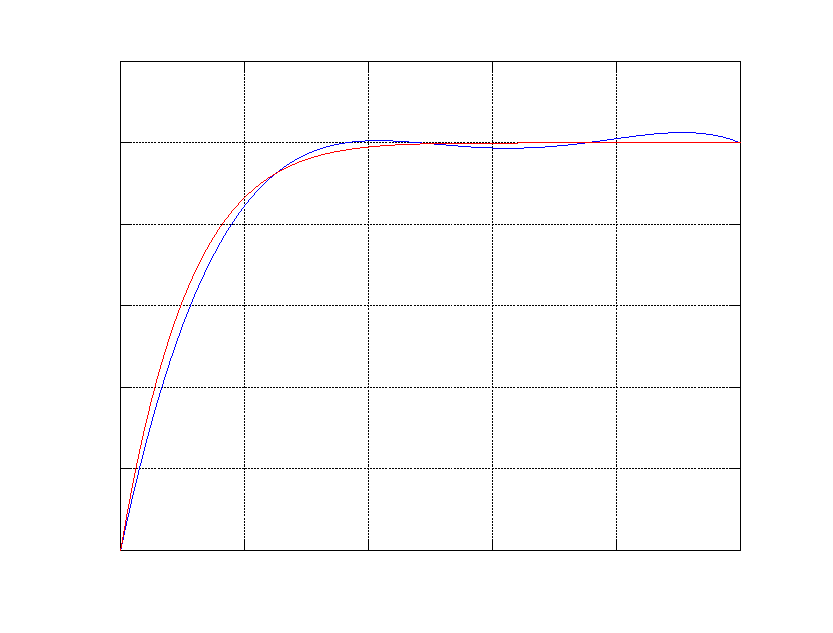
\includegraphics{ApprossimazioneFunzioni/exercise49-normalPlotOutput}}%
    \gplfronttext
  \end{picture}%
\endgroup

\end{center}

Il prossimo plot rappresenta le differenze divise calcolate per costruire i
polinomi interpolanti:
\begin{center} 
% GNUPLOT: LaTeX picture with Postscript
\begingroup
  \makeatletter
  \providecommand\color[2][]{%
    \GenericError{(gnuplot) \space\space\space\@spaces}{%
      Package color not loaded in conjunction with
      terminal option `colourtext'%
    }{See the gnuplot documentation for explanation.%
    }{Either use 'blacktext' in gnuplot or load the package
      color.sty in LaTeX.}%
    \renewcommand\color[2][]{}%
  }%
  \providecommand\includegraphics[2][]{%
    \GenericError{(gnuplot) \space\space\space\@spaces}{%
      Package graphicx or graphics not loaded%
    }{See the gnuplot documentation for explanation.%
    }{The gnuplot epslatex terminal needs graphicx.sty or graphics.sty.}%
    \renewcommand\includegraphics[2][]{}%
  }%
  \providecommand\rotatebox[2]{#2}%
  \@ifundefined{ifGPcolor}{%
    \newif\ifGPcolor
    \GPcolortrue
  }{}%
  \@ifundefined{ifGPblacktext}{%
    \newif\ifGPblacktext
    \GPblacktexttrue
  }{}%
  % define a \g@addto@macro without @ in the name:
  \let\gplgaddtomacro\g@addto@macro
  % define empty templates for all commands taking text:
  \gdef\gplbacktext{}%
  \gdef\gplfronttext{}%
  \makeatother
  \ifGPblacktext
    % no textcolor at all
    \def\colorrgb#1{}%
    \def\colorgray#1{}%
  \else
    % gray or color?
    \ifGPcolor
      \def\colorrgb#1{\color[rgb]{#1}}%
      \def\colorgray#1{\color[gray]{#1}}%
      \expandafter\def\csname LTw\endcsname{\color{white}}%
      \expandafter\def\csname LTb\endcsname{\color{black}}%
      \expandafter\def\csname LTa\endcsname{\color{black}}%
      \expandafter\def\csname LT0\endcsname{\color[rgb]{1,0,0}}%
      \expandafter\def\csname LT1\endcsname{\color[rgb]{0,1,0}}%
      \expandafter\def\csname LT2\endcsname{\color[rgb]{0,0,1}}%
      \expandafter\def\csname LT3\endcsname{\color[rgb]{1,0,1}}%
      \expandafter\def\csname LT4\endcsname{\color[rgb]{0,1,1}}%
      \expandafter\def\csname LT5\endcsname{\color[rgb]{1,1,0}}%
      \expandafter\def\csname LT6\endcsname{\color[rgb]{0,0,0}}%
      \expandafter\def\csname LT7\endcsname{\color[rgb]{1,0.3,0}}%
      \expandafter\def\csname LT8\endcsname{\color[rgb]{0.5,0.5,0.5}}%
    \else
      % gray
      \def\colorrgb#1{\color{black}}%
      \def\colorgray#1{\color[gray]{#1}}%
      \expandafter\def\csname LTw\endcsname{\color{white}}%
      \expandafter\def\csname LTb\endcsname{\color{black}}%
      \expandafter\def\csname LTa\endcsname{\color{black}}%
      \expandafter\def\csname LT0\endcsname{\color{black}}%
      \expandafter\def\csname LT1\endcsname{\color{black}}%
      \expandafter\def\csname LT2\endcsname{\color{black}}%
      \expandafter\def\csname LT3\endcsname{\color{black}}%
      \expandafter\def\csname LT4\endcsname{\color{black}}%
      \expandafter\def\csname LT5\endcsname{\color{black}}%
      \expandafter\def\csname LT6\endcsname{\color{black}}%
      \expandafter\def\csname LT7\endcsname{\color{black}}%
      \expandafter\def\csname LT8\endcsname{\color{black}}%
    \fi
  \fi
  \setlength{\unitlength}{0.0500bp}%
  \begin{picture}(7680.00,5760.00)%
    \gplgaddtomacro\gplbacktext{%
      \colorrgb{0.00,0.00,0.00}%
      \put(866,634){\makebox(0,0)[r]{\strut{}-4000}}%
      \colorrgb{0.00,0.00,0.00}%
      \put(866,1304){\makebox(0,0)[r]{\strut{}-3000}}%
      \colorrgb{0.00,0.00,0.00}%
      \put(866,1975){\makebox(0,0)[r]{\strut{}-2000}}%
      \colorrgb{0.00,0.00,0.00}%
      \put(866,2645){\makebox(0,0)[r]{\strut{}-1000}}%
      \colorrgb{0.00,0.00,0.00}%
      \put(866,3316){\makebox(0,0)[r]{\strut{}0}}%
      \colorrgb{0.00,0.00,0.00}%
      \put(866,3986){\makebox(0,0)[r]{\strut{}1000}}%
      \colorrgb{0.00,0.00,0.00}%
      \put(866,4657){\makebox(0,0)[r]{\strut{}2000}}%
      \colorrgb{0.00,0.00,0.00}%
      \put(866,5327){\makebox(0,0)[r]{\strut{}3000}}%
      \colorrgb{0.00,0.00,0.00}%
      \put(998,414){\makebox(0,0){\strut{}0}}%
      \colorrgb{0.00,0.00,0.00}%
      \put(2188,414){\makebox(0,0){\strut{}0.2}}%
      \colorrgb{0.00,0.00,0.00}%
      \put(3379,414){\makebox(0,0){\strut{}0.4}}%
      \colorrgb{0.00,0.00,0.00}%
      \put(4569,414){\makebox(0,0){\strut{}0.6}}%
      \colorrgb{0.00,0.00,0.00}%
      \put(5760,414){\makebox(0,0){\strut{}0.8}}%
      \colorrgb{0.00,0.00,0.00}%
      \put(6950,414){\makebox(0,0){\strut{}1}}%
    }%
    \gplgaddtomacro\gplfronttext{%
    }%
    \gplbacktext
    \put(0,0){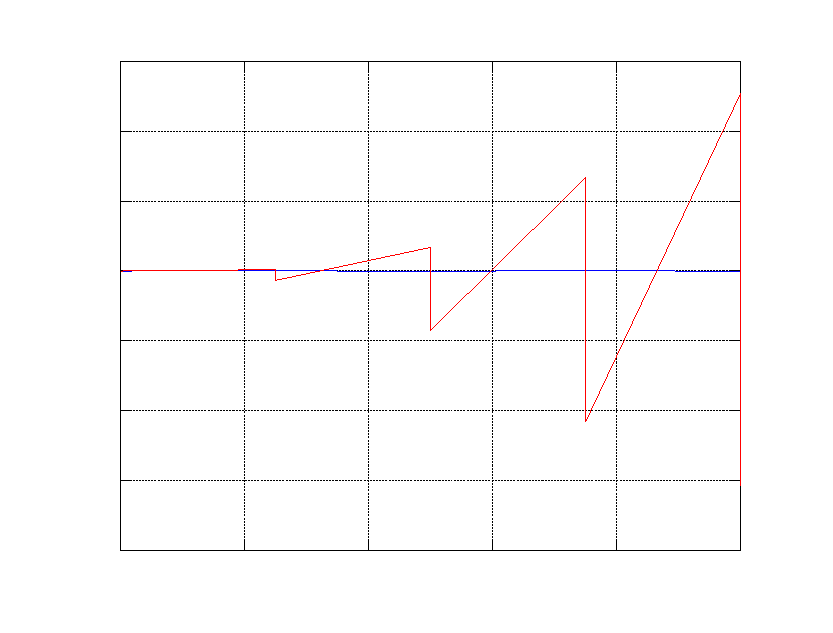
\includegraphics{ApprossimazioneFunzioni/exercise49-DifferenzeDivisePlotOutput}}%
    \gplfronttext
  \end{picture}%
\endgroup

\end{center}

Il prossimo plot mostra gli errori che si commette nelle due approssimazioni,
usando entrambi gli assi con scala lineare:
\begin{center} 
% GNUPLOT: LaTeX picture with Postscript
\begingroup
  \makeatletter
  \providecommand\color[2][]{%
    \GenericError{(gnuplot) \space\space\space\@spaces}{%
      Package color not loaded in conjunction with
      terminal option `colourtext'%
    }{See the gnuplot documentation for explanation.%
    }{Either use 'blacktext' in gnuplot or load the package
      color.sty in LaTeX.}%
    \renewcommand\color[2][]{}%
  }%
  \providecommand\includegraphics[2][]{%
    \GenericError{(gnuplot) \space\space\space\@spaces}{%
      Package graphicx or graphics not loaded%
    }{See the gnuplot documentation for explanation.%
    }{The gnuplot epslatex terminal needs graphicx.sty or graphics.sty.}%
    \renewcommand\includegraphics[2][]{}%
  }%
  \providecommand\rotatebox[2]{#2}%
  \@ifundefined{ifGPcolor}{%
    \newif\ifGPcolor
    \GPcolortrue
  }{}%
  \@ifundefined{ifGPblacktext}{%
    \newif\ifGPblacktext
    \GPblacktexttrue
  }{}%
  % define a \g@addto@macro without @ in the name:
  \let\gplgaddtomacro\g@addto@macro
  % define empty templates for all commands taking text:
  \gdef\gplbacktext{}%
  \gdef\gplfronttext{}%
  \makeatother
  \ifGPblacktext
    % no textcolor at all
    \def\colorrgb#1{}%
    \def\colorgray#1{}%
  \else
    % gray or color?
    \ifGPcolor
      \def\colorrgb#1{\color[rgb]{#1}}%
      \def\colorgray#1{\color[gray]{#1}}%
      \expandafter\def\csname LTw\endcsname{\color{white}}%
      \expandafter\def\csname LTb\endcsname{\color{black}}%
      \expandafter\def\csname LTa\endcsname{\color{black}}%
      \expandafter\def\csname LT0\endcsname{\color[rgb]{1,0,0}}%
      \expandafter\def\csname LT1\endcsname{\color[rgb]{0,1,0}}%
      \expandafter\def\csname LT2\endcsname{\color[rgb]{0,0,1}}%
      \expandafter\def\csname LT3\endcsname{\color[rgb]{1,0,1}}%
      \expandafter\def\csname LT4\endcsname{\color[rgb]{0,1,1}}%
      \expandafter\def\csname LT5\endcsname{\color[rgb]{1,1,0}}%
      \expandafter\def\csname LT6\endcsname{\color[rgb]{0,0,0}}%
      \expandafter\def\csname LT7\endcsname{\color[rgb]{1,0.3,0}}%
      \expandafter\def\csname LT8\endcsname{\color[rgb]{0.5,0.5,0.5}}%
    \else
      % gray
      \def\colorrgb#1{\color{black}}%
      \def\colorgray#1{\color[gray]{#1}}%
      \expandafter\def\csname LTw\endcsname{\color{white}}%
      \expandafter\def\csname LTb\endcsname{\color{black}}%
      \expandafter\def\csname LTa\endcsname{\color{black}}%
      \expandafter\def\csname LT0\endcsname{\color{black}}%
      \expandafter\def\csname LT1\endcsname{\color{black}}%
      \expandafter\def\csname LT2\endcsname{\color{black}}%
      \expandafter\def\csname LT3\endcsname{\color{black}}%
      \expandafter\def\csname LT4\endcsname{\color{black}}%
      \expandafter\def\csname LT5\endcsname{\color{black}}%
      \expandafter\def\csname LT6\endcsname{\color{black}}%
      \expandafter\def\csname LT7\endcsname{\color{black}}%
      \expandafter\def\csname LT8\endcsname{\color{black}}%
    \fi
  \fi
  \setlength{\unitlength}{0.0500bp}%
  \begin{picture}(7680.00,5760.00)%
    \gplgaddtomacro\gplbacktext{%
      \colorrgb{0.00,0.00,0.00}%
      \put(866,634){\makebox(0,0)[r]{\strut{}0}}%
      \colorrgb{0.00,0.00,0.00}%
      \put(866,1221){\makebox(0,0)[r]{\strut{}0.01}}%
      \colorrgb{0.00,0.00,0.00}%
      \put(866,1807){\makebox(0,0)[r]{\strut{}0.02}}%
      \colorrgb{0.00,0.00,0.00}%
      \put(866,2394){\makebox(0,0)[r]{\strut{}0.03}}%
      \colorrgb{0.00,0.00,0.00}%
      \put(866,2981){\makebox(0,0)[r]{\strut{}0.04}}%
      \colorrgb{0.00,0.00,0.00}%
      \put(866,3567){\makebox(0,0)[r]{\strut{}0.05}}%
      \colorrgb{0.00,0.00,0.00}%
      \put(866,4154){\makebox(0,0)[r]{\strut{}0.06}}%
      \colorrgb{0.00,0.00,0.00}%
      \put(866,4740){\makebox(0,0)[r]{\strut{}0.07}}%
      \colorrgb{0.00,0.00,0.00}%
      \put(866,5327){\makebox(0,0)[r]{\strut{}0.08}}%
      \colorrgb{0.00,0.00,0.00}%
      \put(998,414){\makebox(0,0){\strut{}0}}%
      \colorrgb{0.00,0.00,0.00}%
      \put(2188,414){\makebox(0,0){\strut{}0.2}}%
      \colorrgb{0.00,0.00,0.00}%
      \put(3379,414){\makebox(0,0){\strut{}0.4}}%
      \colorrgb{0.00,0.00,0.00}%
      \put(4569,414){\makebox(0,0){\strut{}0.6}}%
      \colorrgb{0.00,0.00,0.00}%
      \put(5760,414){\makebox(0,0){\strut{}0.8}}%
      \colorrgb{0.00,0.00,0.00}%
      \put(6950,414){\makebox(0,0){\strut{}1}}%
    }%
    \gplgaddtomacro\gplfronttext{%
    }%
    \gplbacktext
    \put(0,0){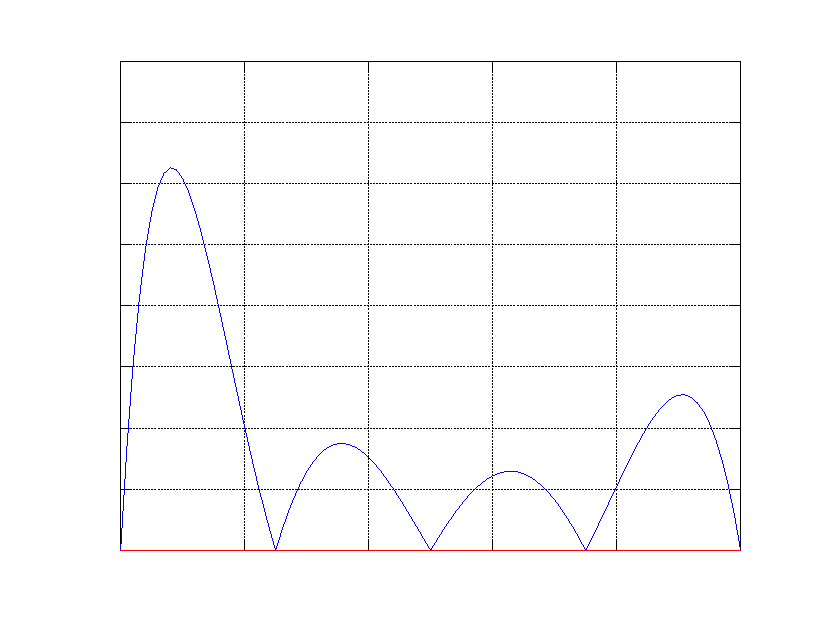
\includegraphics{ApprossimazioneFunzioni/exercise49-errorsPlotOutput}}%
    \gplfronttext
  \end{picture}%
\endgroup

\end{center}

Il prossimo plot mostra gli errori che si commette nelle due approssimazioni,
usando l'asse delle ordinate con scala logaritmica, in modo da evidenziare che
anche usando lo schema di \emph{Hermite} si commettono errori, molto piccoli,
ma che non era possibile apprezzarli nel plot precedente:
\begin{center} 
% GNUPLOT: LaTeX picture with Postscript
\begingroup
  \makeatletter
  \providecommand\color[2][]{%
    \GenericError{(gnuplot) \space\space\space\@spaces}{%
      Package color not loaded in conjunction with
      terminal option `colourtext'%
    }{See the gnuplot documentation for explanation.%
    }{Either use 'blacktext' in gnuplot or load the package
      color.sty in LaTeX.}%
    \renewcommand\color[2][]{}%
  }%
  \providecommand\includegraphics[2][]{%
    \GenericError{(gnuplot) \space\space\space\@spaces}{%
      Package graphicx or graphics not loaded%
    }{See the gnuplot documentation for explanation.%
    }{The gnuplot epslatex terminal needs graphicx.sty or graphics.sty.}%
    \renewcommand\includegraphics[2][]{}%
  }%
  \providecommand\rotatebox[2]{#2}%
  \@ifundefined{ifGPcolor}{%
    \newif\ifGPcolor
    \GPcolortrue
  }{}%
  \@ifundefined{ifGPblacktext}{%
    \newif\ifGPblacktext
    \GPblacktexttrue
  }{}%
  % define a \g@addto@macro without @ in the name:
  \let\gplgaddtomacro\g@addto@macro
  % define empty templates for all commands taking text:
  \gdef\gplbacktext{}%
  \gdef\gplfronttext{}%
  \makeatother
  \ifGPblacktext
    % no textcolor at all
    \def\colorrgb#1{}%
    \def\colorgray#1{}%
  \else
    % gray or color?
    \ifGPcolor
      \def\colorrgb#1{\color[rgb]{#1}}%
      \def\colorgray#1{\color[gray]{#1}}%
      \expandafter\def\csname LTw\endcsname{\color{white}}%
      \expandafter\def\csname LTb\endcsname{\color{black}}%
      \expandafter\def\csname LTa\endcsname{\color{black}}%
      \expandafter\def\csname LT0\endcsname{\color[rgb]{1,0,0}}%
      \expandafter\def\csname LT1\endcsname{\color[rgb]{0,1,0}}%
      \expandafter\def\csname LT2\endcsname{\color[rgb]{0,0,1}}%
      \expandafter\def\csname LT3\endcsname{\color[rgb]{1,0,1}}%
      \expandafter\def\csname LT4\endcsname{\color[rgb]{0,1,1}}%
      \expandafter\def\csname LT5\endcsname{\color[rgb]{1,1,0}}%
      \expandafter\def\csname LT6\endcsname{\color[rgb]{0,0,0}}%
      \expandafter\def\csname LT7\endcsname{\color[rgb]{1,0.3,0}}%
      \expandafter\def\csname LT8\endcsname{\color[rgb]{0.5,0.5,0.5}}%
    \else
      % gray
      \def\colorrgb#1{\color{black}}%
      \def\colorgray#1{\color[gray]{#1}}%
      \expandafter\def\csname LTw\endcsname{\color{white}}%
      \expandafter\def\csname LTb\endcsname{\color{black}}%
      \expandafter\def\csname LTa\endcsname{\color{black}}%
      \expandafter\def\csname LT0\endcsname{\color{black}}%
      \expandafter\def\csname LT1\endcsname{\color{black}}%
      \expandafter\def\csname LT2\endcsname{\color{black}}%
      \expandafter\def\csname LT3\endcsname{\color{black}}%
      \expandafter\def\csname LT4\endcsname{\color{black}}%
      \expandafter\def\csname LT5\endcsname{\color{black}}%
      \expandafter\def\csname LT6\endcsname{\color{black}}%
      \expandafter\def\csname LT7\endcsname{\color{black}}%
      \expandafter\def\csname LT8\endcsname{\color{black}}%
    \fi
  \fi
  \setlength{\unitlength}{0.0500bp}%
  \begin{picture}(7680.00,5760.00)%
    \gplgaddtomacro\gplbacktext{%
      \colorrgb{0.00,0.00,0.00}%
      \put(866,634){\makebox(0,0)[r]{\strut{}$10^{-20}$}}%
      \colorrgb{0.00,0.00,0.00}%
      \put(866,1807){\makebox(0,0)[r]{\strut{}$10^{-15}$}}%
      \colorrgb{0.00,0.00,0.00}%
      \put(866,2981){\makebox(0,0)[r]{\strut{}$10^{-10}$}}%
      \colorrgb{0.00,0.00,0.00}%
      \put(866,4154){\makebox(0,0)[r]{\strut{}$10^{-5}$}}%
      \colorrgb{0.00,0.00,0.00}%
      \put(866,5327){\makebox(0,0)[r]{\strut{}$10^{0}$}}%
      \colorrgb{0.00,0.00,0.00}%
      \put(998,414){\makebox(0,0){\strut{}0}}%
      \colorrgb{0.00,0.00,0.00}%
      \put(2188,414){\makebox(0,0){\strut{}0.2}}%
      \colorrgb{0.00,0.00,0.00}%
      \put(3379,414){\makebox(0,0){\strut{}0.4}}%
      \colorrgb{0.00,0.00,0.00}%
      \put(4569,414){\makebox(0,0){\strut{}0.6}}%
      \colorrgb{0.00,0.00,0.00}%
      \put(5760,414){\makebox(0,0){\strut{}0.8}}%
      \colorrgb{0.00,0.00,0.00}%
      \put(6950,414){\makebox(0,0){\strut{}1}}%
    }%
    \gplgaddtomacro\gplfronttext{%
    }%
    \gplbacktext
    \put(0,0){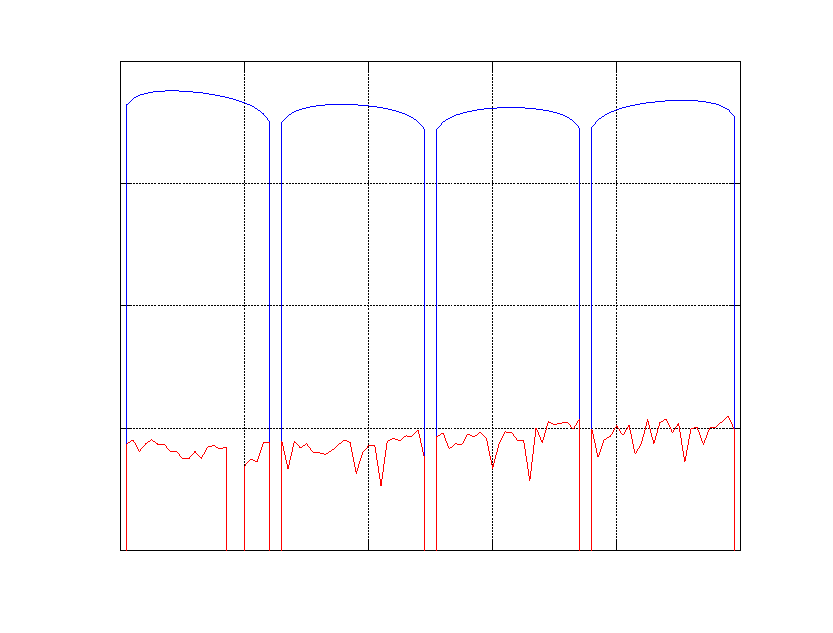
\includegraphics{ApprossimazioneFunzioni/exercise49-errorsSemilogYPlotOutput}}%
    \gplfronttext
  \end{picture}%
\endgroup

\end{center}

\begin{exercise}[4.11]
\label{exercise:exercise411}
Per il testo dell'esercizio consultare il libro di testo.
\end{exercise}
Per il codice che implementa le richieste dell'esercizio e produce i seguenti
risultati vedere \nameref{subsec:exercise411}.

Nei seguenti grafici in
\emph{rosso} \`e rappresentata la funzione di \emph{Bernstein}, mentre in \emph{blu} \`e rappresentata la funzione di
\emph{Runge}. Questo primo grafico ha l'asse delle ordinate costruito in
modo logaritmico:
\begin{center}   
% GNUPLOT: LaTeX picture with Postscript
\begingroup
  \makeatletter
  \providecommand\color[2][]{%
    \GenericError{(gnuplot) \space\space\space\@spaces}{%
      Package color not loaded in conjunction with
      terminal option `colourtext'%
    }{See the gnuplot documentation for explanation.%
    }{Either use 'blacktext' in gnuplot or load the package
      color.sty in LaTeX.}%
    \renewcommand\color[2][]{}%
  }%
  \providecommand\includegraphics[2][]{%
    \GenericError{(gnuplot) \space\space\space\@spaces}{%
      Package graphicx or graphics not loaded%
    }{See the gnuplot documentation for explanation.%
    }{The gnuplot epslatex terminal needs graphicx.sty or graphics.sty.}%
    \renewcommand\includegraphics[2][]{}%
  }%
  \providecommand\rotatebox[2]{#2}%
  \@ifundefined{ifGPcolor}{%
    \newif\ifGPcolor
    \GPcolortrue
  }{}%
  \@ifundefined{ifGPblacktext}{%
    \newif\ifGPblacktext
    \GPblacktexttrue
  }{}%
  % define a \g@addto@macro without @ in the name:
  \let\gplgaddtomacro\g@addto@macro
  % define empty templates for all commands taking text:
  \gdef\gplbacktext{}%
  \gdef\gplfronttext{}%
  \makeatother
  \ifGPblacktext
    % no textcolor at all
    \def\colorrgb#1{}%
    \def\colorgray#1{}%
  \else
    % gray or color?
    \ifGPcolor
      \def\colorrgb#1{\color[rgb]{#1}}%
      \def\colorgray#1{\color[gray]{#1}}%
      \expandafter\def\csname LTw\endcsname{\color{white}}%
      \expandafter\def\csname LTb\endcsname{\color{black}}%
      \expandafter\def\csname LTa\endcsname{\color{black}}%
      \expandafter\def\csname LT0\endcsname{\color[rgb]{1,0,0}}%
      \expandafter\def\csname LT1\endcsname{\color[rgb]{0,1,0}}%
      \expandafter\def\csname LT2\endcsname{\color[rgb]{0,0,1}}%
      \expandafter\def\csname LT3\endcsname{\color[rgb]{1,0,1}}%
      \expandafter\def\csname LT4\endcsname{\color[rgb]{0,1,1}}%
      \expandafter\def\csname LT5\endcsname{\color[rgb]{1,1,0}}%
      \expandafter\def\csname LT6\endcsname{\color[rgb]{0,0,0}}%
      \expandafter\def\csname LT7\endcsname{\color[rgb]{1,0.3,0}}%
      \expandafter\def\csname LT8\endcsname{\color[rgb]{0.5,0.5,0.5}}%
    \else
      % gray
      \def\colorrgb#1{\color{black}}%
      \def\colorgray#1{\color[gray]{#1}}%
      \expandafter\def\csname LTw\endcsname{\color{white}}%
      \expandafter\def\csname LTb\endcsname{\color{black}}%
      \expandafter\def\csname LTa\endcsname{\color{black}}%
      \expandafter\def\csname LT0\endcsname{\color{black}}%
      \expandafter\def\csname LT1\endcsname{\color{black}}%
      \expandafter\def\csname LT2\endcsname{\color{black}}%
      \expandafter\def\csname LT3\endcsname{\color{black}}%
      \expandafter\def\csname LT4\endcsname{\color{black}}%
      \expandafter\def\csname LT5\endcsname{\color{black}}%
      \expandafter\def\csname LT6\endcsname{\color{black}}%
      \expandafter\def\csname LT7\endcsname{\color{black}}%
      \expandafter\def\csname LT8\endcsname{\color{black}}%
    \fi
  \fi
  \setlength{\unitlength}{0.0500bp}%
  \begin{picture}(7680.00,5760.00)%
    \gplgaddtomacro\gplbacktext{%
      \colorrgb{0.00,0.00,0.00}%
      \put(866,634){\makebox(0,0)[r]{\strut{}$10^{-5}$}}%
      \colorrgb{0.00,0.00,0.00}%
      \put(866,1416){\makebox(0,0)[r]{\strut{}$10^{0}$}}%
      \colorrgb{0.00,0.00,0.00}%
      \put(866,2198){\makebox(0,0)[r]{\strut{}$10^{5}$}}%
      \colorrgb{0.00,0.00,0.00}%
      \put(866,2981){\makebox(0,0)[r]{\strut{}$10^{10}$}}%
      \colorrgb{0.00,0.00,0.00}%
      \put(866,3763){\makebox(0,0)[r]{\strut{}$10^{15}$}}%
      \colorrgb{0.00,0.00,0.00}%
      \put(866,4545){\makebox(0,0)[r]{\strut{}$10^{20}$}}%
      \colorrgb{0.00,0.00,0.00}%
      \put(866,5327){\makebox(0,0)[r]{\strut{}$10^{25}$}}%
      \colorrgb{0.00,0.00,0.00}%
      \put(998,414){\makebox(0,0){\strut{}0}}%
      \colorrgb{0.00,0.00,0.00}%
      \put(2188,414){\makebox(0,0){\strut{}20}}%
      \colorrgb{0.00,0.00,0.00}%
      \put(3379,414){\makebox(0,0){\strut{}40}}%
      \colorrgb{0.00,0.00,0.00}%
      \put(4569,414){\makebox(0,0){\strut{}60}}%
      \colorrgb{0.00,0.00,0.00}%
      \put(5760,414){\makebox(0,0){\strut{}80}}%
      \colorrgb{0.00,0.00,0.00}%
      \put(6950,414){\makebox(0,0){\strut{}100}}%
    }%
    \gplgaddtomacro\gplfronttext{%
    }%
    \gplbacktext
    \put(0,0){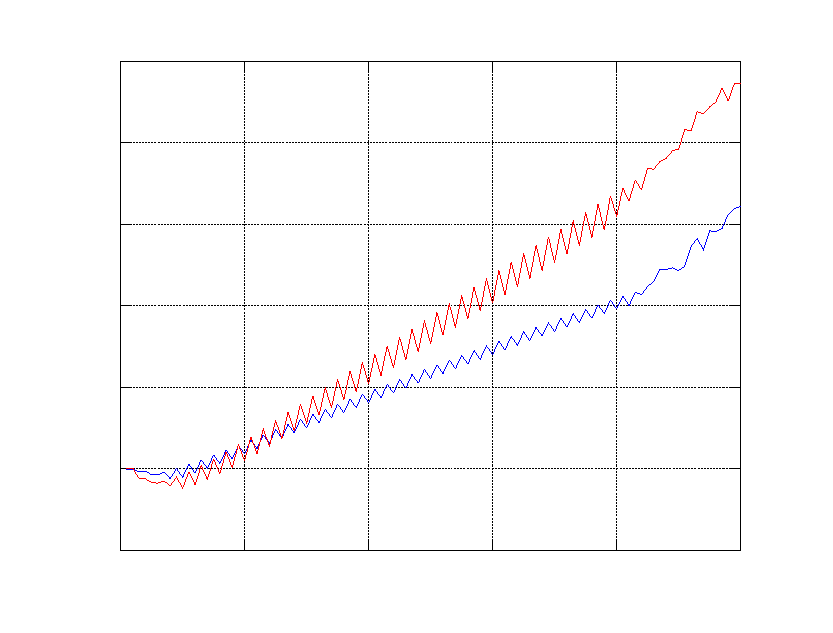
\includegraphics{ApprossimazioneFunzioni/exercise411-ErrorsSemilogYPlotOutput}}%
    \gplfronttext
  \end{picture}%
\endgroup

\end{center}
Riporto lo stesso dataset di errori per le due curve, costruendo entrambi gli
assi in modo logaritmico:
\begin{center}  
% GNUPLOT: LaTeX picture with Postscript
\begingroup
  \makeatletter
  \providecommand\color[2][]{%
    \GenericError{(gnuplot) \space\space\space\@spaces}{%
      Package color not loaded in conjunction with
      terminal option `colourtext'%
    }{See the gnuplot documentation for explanation.%
    }{Either use 'blacktext' in gnuplot or load the package
      color.sty in LaTeX.}%
    \renewcommand\color[2][]{}%
  }%
  \providecommand\includegraphics[2][]{%
    \GenericError{(gnuplot) \space\space\space\@spaces}{%
      Package graphicx or graphics not loaded%
    }{See the gnuplot documentation for explanation.%
    }{The gnuplot epslatex terminal needs graphicx.sty or graphics.sty.}%
    \renewcommand\includegraphics[2][]{}%
  }%
  \providecommand\rotatebox[2]{#2}%
  \@ifundefined{ifGPcolor}{%
    \newif\ifGPcolor
    \GPcolortrue
  }{}%
  \@ifundefined{ifGPblacktext}{%
    \newif\ifGPblacktext
    \GPblacktexttrue
  }{}%
  % define a \g@addto@macro without @ in the name:
  \let\gplgaddtomacro\g@addto@macro
  % define empty templates for all commands taking text:
  \gdef\gplbacktext{}%
  \gdef\gplfronttext{}%
  \makeatother
  \ifGPblacktext
    % no textcolor at all
    \def\colorrgb#1{}%
    \def\colorgray#1{}%
  \else
    % gray or color?
    \ifGPcolor
      \def\colorrgb#1{\color[rgb]{#1}}%
      \def\colorgray#1{\color[gray]{#1}}%
      \expandafter\def\csname LTw\endcsname{\color{white}}%
      \expandafter\def\csname LTb\endcsname{\color{black}}%
      \expandafter\def\csname LTa\endcsname{\color{black}}%
      \expandafter\def\csname LT0\endcsname{\color[rgb]{1,0,0}}%
      \expandafter\def\csname LT1\endcsname{\color[rgb]{0,1,0}}%
      \expandafter\def\csname LT2\endcsname{\color[rgb]{0,0,1}}%
      \expandafter\def\csname LT3\endcsname{\color[rgb]{1,0,1}}%
      \expandafter\def\csname LT4\endcsname{\color[rgb]{0,1,1}}%
      \expandafter\def\csname LT5\endcsname{\color[rgb]{1,1,0}}%
      \expandafter\def\csname LT6\endcsname{\color[rgb]{0,0,0}}%
      \expandafter\def\csname LT7\endcsname{\color[rgb]{1,0.3,0}}%
      \expandafter\def\csname LT8\endcsname{\color[rgb]{0.5,0.5,0.5}}%
    \else
      % gray
      \def\colorrgb#1{\color{black}}%
      \def\colorgray#1{\color[gray]{#1}}%
      \expandafter\def\csname LTw\endcsname{\color{white}}%
      \expandafter\def\csname LTb\endcsname{\color{black}}%
      \expandafter\def\csname LTa\endcsname{\color{black}}%
      \expandafter\def\csname LT0\endcsname{\color{black}}%
      \expandafter\def\csname LT1\endcsname{\color{black}}%
      \expandafter\def\csname LT2\endcsname{\color{black}}%
      \expandafter\def\csname LT3\endcsname{\color{black}}%
      \expandafter\def\csname LT4\endcsname{\color{black}}%
      \expandafter\def\csname LT5\endcsname{\color{black}}%
      \expandafter\def\csname LT6\endcsname{\color{black}}%
      \expandafter\def\csname LT7\endcsname{\color{black}}%
      \expandafter\def\csname LT8\endcsname{\color{black}}%
    \fi
  \fi
  \setlength{\unitlength}{0.0500bp}%
  \begin{picture}(7680.00,5760.00)%
    \gplgaddtomacro\gplbacktext{%
      \colorrgb{0.00,0.00,0.00}%
      \put(866,633){\makebox(0,0)[r]{\strut{}$10^{-2}$}}%
      \colorrgb{0.00,0.00,0.00}%
      \put(866,1415){\makebox(0,0)[r]{\strut{}$10^{0}$}}%
      \colorrgb{0.00,0.00,0.00}%
      \put(866,2198){\makebox(0,0)[r]{\strut{}$10^{2}$}}%
      \colorrgb{0.00,0.00,0.00}%
      \put(866,2980){\makebox(0,0)[r]{\strut{}$10^{4}$}}%
      \colorrgb{0.00,0.00,0.00}%
      \put(866,3762){\makebox(0,0)[r]{\strut{}$10^{6}$}}%
      \colorrgb{0.00,0.00,0.00}%
      \put(866,4545){\makebox(0,0)[r]{\strut{}$10^{8}$}}%
      \colorrgb{0.00,0.00,0.00}%
      \put(866,5327){\makebox(0,0)[r]{\strut{}$10^{10}$}}%
      \colorrgb{0.00,0.00,0.00}%
      \put(998,413){\makebox(0,0){\strut{}$10^{0}$}}%
      \colorrgb{0.00,0.00,0.00}%
      \put(3974,413){\makebox(0,0){\strut{}$10^{1}$}}%
      \colorrgb{0.00,0.00,0.00}%
      \put(6949,413){\makebox(0,0){\strut{}$10^{2}$}}%
    }%
    \gplgaddtomacro\gplfronttext{%
    }%
    \gplbacktext
    \put(0,0){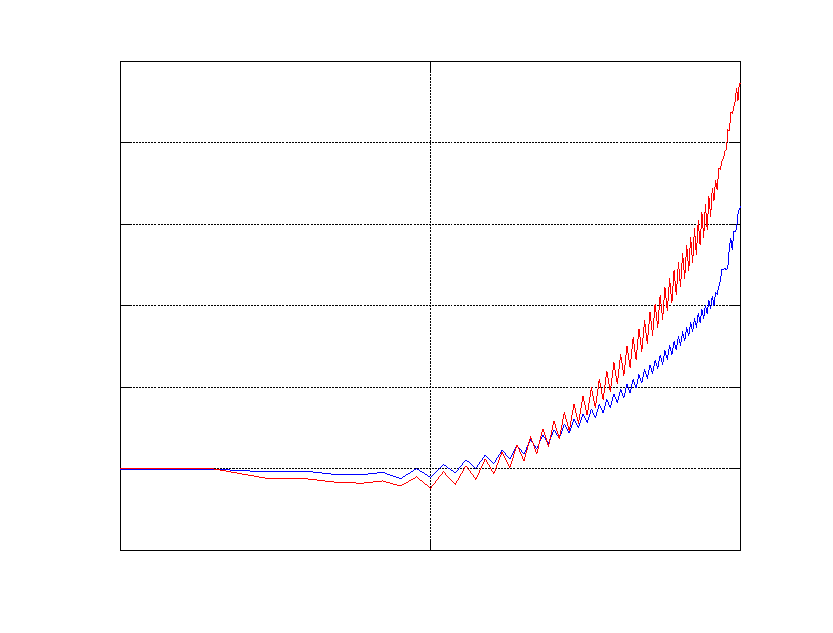
\includegraphics{ApprossimazioneFunzioni/exercise411-ErrorsLoglogPlotOutput}}%
    \gplfronttext
  \end{picture}%
\endgroup

\end{center}
Per entrambi i grafici, le valutazioni della rispettiva funzione, del polinomio
interpolante e la costruzione del polinomio interpolante sono riferiti ai
rispettivi dominii $[a,b]$ definiti nel testo dell'esercizio.

Possiamo notare che l'errore diverge all'aumentare del numero di ascisse di
interpolazione e, confrontando gli errori ottenuti per le due funzioni, possiamo
dire il problema di interpolare la funzione di \emph{Bernstein} \`e maggiormente
malcondizionato del problema di interpolare la funzione di \emph{Runge}.

\begin{exercise}[4.12]
\label{exercise:exercise412}
Per il testo dell'esercizio consultare il libro di testo.
\end{exercise}
\begin{proof}
	Dimostro i due versi distinti di:
	\begin{displaymath}
	x \in [-1,1] \Leftrightarrow \tilde{x} = \tilde{x}(x) \in
	[a, b] \quad \text{con } \tilde{x} = \tilde{x}(x) = \frac{a + b}{2} +
	\frac{b-a}{2}x
	\end{displaymath}
	supponendo senza perdere di generalit\`a $a \leq b$:
	\begin{itemize}
	  \item $(\Rightarrow)$ Quello che voglio utilizzare \`e $\tilde{x} =
	  \tilde{x}(x)$
		\begin{itemize}
	  		\item se $x = -1$:
	  		\begin{displaymath}
	  			\tilde{x}(x) = \frac{a + b}{2} - \frac{b-a}{2} = 
	  			\frac{a + b - b +a}{2} = a \in [a,b]
	  		\end{displaymath}
	  		vero perch\`e $a \leq b$ per ipotesi.
	  		\item se $x = 1$:
	  		\begin{displaymath}
	  			\tilde{x}(x) = \frac{a + b}{2} + \frac{b-a}{2} = 
	  			\frac{a + b + b -a}{2} = b \in [a,b]
	  		\end{displaymath}
	  		vero perch\`e $a \leq b$ per ipotesi.
	  		\item se $x = 0$:
	  		\begin{displaymath}
	  			\tilde{x}(x) = \frac{a + b}{2} 
	  		\end{displaymath}
	  		per ipotesi $a \leq b$ allora $\exists \epsilon \geq 0: b = a + \epsilon$,
	  		quindi ottengo:
	  		\begin{displaymath}
	  			\tilde{x}(x) = \frac{a + b}{2} = \frac{2a + \epsilon}{2} =
	  				a + \frac{\epsilon}{2}   
	  		\end{displaymath}
	  		Ma $a + \frac{\epsilon}{2} \geq a$ perch\`e $\frac{\epsilon}{2} \geq 0$ 
	  		in quanto $\epsilon \geq 0$ per ipotesi.
	  		
	  		Ma $a + \frac{\epsilon}{2} \leq b$ perch\`e $b = a + \epsilon$ implica
	  		$a + \frac{\epsilon}{2} \leq a + \epsilon$, vero perch\`e
	  		$\frac{\epsilon}{2} \leq \epsilon$ in quanto $\epsilon \geq 0$ per ipotesi.
	  		Quindi $\tilde{x}(x) \in [a,b]$.
		\end{itemize}  
		
	 \item $(\Leftarrow)$ Quello che voglio utilizzare \`e $x =
	  x(\tilde{x})$. Dalle ipotesi segue che:
	 \begin{displaymath}
	 \begin{split}
	 	\tilde{x} &= \frac{a+b}{2} + \frac{b-a}{2}x \\
	 	2\tilde{x} &= a + b + (b-a) x \\
	 	2\tilde{x} &= a + (b -a) +a +(b-a)x \\
	 	2(\tilde{x} -a) &= (b-a)(x+1) \\
	 	\frac{2(\tilde{x} -a)}{b-a} &= x+1 \\
	 	\frac{2(\tilde{x} -a)}{b-a} -1 &= x
	 \end{split}
	 \end{displaymath}
	 
	 Se $\tilde{x} = \min\{[a,b]\} = a \Rightarrow x = -1$.
	 
	 Se $\tilde{x} = \max\{[a,b]\} = a \Rightarrow x = \frac{2(b-a)}{(b-a)}-1 = 1$
	 
	 $x(\tilde{x}) = 0$ per $2\tilde{x} -2a + a -b = 0$ quindi per $\tilde{x} =
	 \frac{b+a}{2}$. Inoltre $x'(\tilde{x}) = \frac{2}{b-a}$, la derivata prima \`e
	 costante, non ci sono punti di min o max locali. Quindi $x \in [-1,1]$.
	\end{itemize}
\end{proof}

\begin{exercise}
Sia $f \in \mathcal{C}^{(1)}([a,b])$ una funzione \emph{Lipschtziana}. Allora $L
= ||f^{(1)}||$.
\end{exercise}
\begin{proof}
Per ipotesi $f$ \`e \emph{Lipschtziana}, quindi vale $|f(x) - f(y)| \leq
L|x-y|, \forall L < \infty, \forall x,y \in [a,b]$. Inoltre $f \in
\mathcal{C}^{(1)}([a,b])$, allora posso scrivere un suo sviluppo di Taylor
$T_{f_{y}}(x)$ centrato in $y$ del termine $f(x)$, con resto al secondo ordine: 
$f(x) = T_{f_{y}}(x) = f(y) + f^{(1)}(y)(x-y) +
\frac{f^{(2)}(\xi)}{2}(x-y)^{2}$, con $\xi \in [x,y]$. Quindi posso utilizzare
questo sviluppo nella propriet\`a di $f$ di essere  \emph{Lipschtziana}:
\begin{displaymath}
\begin{split}
	|f(x) - f(y)| &\leq L|x-y| \\
	|T_{f_{y}}(x) - f(y)| &\leq L|x-y| \\
	|f(y) + f^{(1)}(y)(x-y) - f(y)| &\leq L|x-y| \quad \text{ ho approssimato non
	considerando il resto} \\
	|f^{(1)}(y)(x-y)| &\leq L|x-y| \\
	|f^{(1)}(y)| |x-y| &\leq L|x-y| \\
	|f^{(1)}(y)| &\leq L \\
	||f^{(1)}|| = \max_{y \in [a,b]}{|f^{(1)}(y)|} &= L 
\end{split}
\end{displaymath}
Nell'ultimo passaggio ho cambiato la relazione $\leq$ in $=$, in quanto
considerando la norma cerco il valore massimo.
\end{proof}

\begin{exercise}
Sia $f \in \mathcal{C}^{(1)}([a,b])$ una funzione \emph{Lipschtziana}. Allora 
$w(f;h) \leq Lh$, con $h>0$.
\end{exercise}
\begin{proof}
Dalla definizione di $f$ \emph{Lipschtziana} segue che 
\begin{displaymath}
\begin{split}
	|f(x) - f(y)| &\leq L|x-y| \\
	\max_{x,y \in [a,b]}\{|f(x) - f(y)|\} &\leq \max_{x,y \in [a,b]}\{L|x-y|\}
	\quad \text{ho applicato la funzione $\max$ ad entrambi i membri}\\
	\max_{x,y \in [a,b]}\{|f(x) - f(y)|\} &\leq L \max_{x,y \in [a,b]}\{|x-y|\} \\
	\max_{x,y \in [a,b]}\{|f(x) - f(y)|:|x-y| < h\} &\leq L \max_{x,y \in
	[a,b]}\{|x-y|:|x-y| < h\} \quad \text{impongo vincolo sulla distanza $|x-y|$}\\
	w(f;h) \leq Lh
\end{split}
\end{displaymath}
\end{proof}

\begin{exercise}
Dimostrare che al crescere di $n$ il termine $w(f;\frac{b-a}{n}) \rightarrow 0$.
\end{exercise}
\begin{proof}
Per ipotesi segue che $h = \frac{b-a}{n} \rightarrow 0$. 
\\Posso usare le definizione di $w(f;h) = \sup\{|f(x) - f(y)|:\exists h > 0:
|x-y| < h\}$. 
\\Istanzio per il nostro caso di $h \rightarrow 0$ ottenendo $w(f;h) = 
\sup\{|f(x) - f(y)|:h \rightarrow 0\}$.
\\ Supponendo $f$ continua allora vale $ \lim_{x \rightarrow y}{f(x) = f(y)}$.
\\ Compongo questi risultati:
\begin{displaymath}
\lim_{h \rightarrow 0}{w(f;h)} = \lim_{h \rightarrow 0}{\sup\{|f(x) -
f(y)|:|x-y| = h\}} = \lim_{x \rightarrow y}{\sup\{|f(x) - f(y)|\}} = \lim_{x
\rightarrow y}{\sup\{|f(y) - f(y)|\}} = 0
\end{displaymath}
\end{proof}

\begin{exercise}
\label{exercise:ChebyshevPolyProperties}
Dimostrare le propriet\`a dei polinomi di \emph{Chebyshev} di pagina 92.
\end{exercise}
\begin{proof}
Dimostro per punti:
\begin{enumerate}
  \item $T_{k}(x)$ ha grado esatto $k$
  
  \paragraph{Proof} Prova per induzione su $k$.
  \begin{description}
  \item[Base] per $k = 0$ si ha per la definizione dei polinomi di
  \emph{Chebyshev}, $T_{0}(x) = 1$, essendo una costante implica $\deg(T_{0}(x))
  = 0$, la base \`e vera.
  \item[Induction HP] suppongo vero che $\deg(T_{k-1}(x)) = k-1$ e
  $\deg(T_{k-2}(x)) = k-2$
  \item[Induction step] dimostro per $k$:
  \\ dalla definizione del $k$-esimo polinomio: $T_{k}(x) = 2 x T_{k-1}(x) -
  T_{k-2}(x)$
  \\ Applico la funzione $\deg$ ad entrambi i membri: $\deg(T_{k}(x)) = \deg(2 x
  T_{k-1}(x) - T_{k-2}(x))$
  \\ La funzione $\deg$ applicata ad una somma di polinomi produce: 
   \begin{displaymath}
   \begin{split}
   \deg(2 x  T_{k-1}(x) - T_{k-2}(x)) &= \max\{\deg(2 x
   T_{k-1}(x)), \deg(T_{k-2}(x))\} = \\
    &= \max\{\deg(2x) + \deg(T_{k-1}(x)),
   \deg(T_{k-2}(x)) \}
	\end{split}
	\end{displaymath}
 Ma per ipotesi induttiva: $\deg(T_{k-1}(x)) = k-1 > k-2 = \deg(T_{k-2}(x))$,
 quindi:
 \begin{displaymath}
   \begin{split}
   	\max\{\deg(2x) + \deg(T_{k-1}(x)), \deg(T_{k-2}(x)) \} &= \deg(2x) +
   	\deg(T_{k-1}(x)) = 1 + (k-1) = k
	\end{split}
	\end{displaymath}
	
	
  \end{description}
  
  \item Il coefficiente principale di $T_{k}(x)$, in simboli $cp(T_{k}(x))$,
  soddisfa $cp(T_{k}(x)) = 2^{k-1}, k \geq 1$
  
  \paragraph{Proof} Prova per induzione su $k$.
  \begin{description}
  \item[Base] per $k = 1$ si ha per la definizione dei polinomi di
  \emph{Chebyshev}, $T_{1}(x) = x$, quindi $cp(x) = 1 = 2^{1-1} = 1$,  la base
  \`e vera.
  \item[Induction HP] suppongo vero che $cp(T_{k-1}(x)) = 2^{k-2}$,
  $cp(T_{k-2}(x)) = 2^{k-3}$
  \item[Induction step] dimostro per $k$:
  \\ dalla definizione del $k$-esimo polinomio: $T_{k}(x) = 2 x T_{k-1}(x) -
  T_{k-2}(x)$
  \\ Applico la funzione $cp$ ad entrambi i membri: $cp(T_{k}(x)) = cp(2 x
  T_{k-1}(x) - T_{k-2}(x))$
  \\ La funzione $cp$ applicata ad una somma di polinomi produce: 
   \begin{displaymath}
   \begin{split}
   cp(2 x  T_{k-1}(x) - T_{k-2}(x)) &= \max\{cp(2 x
   T_{k-1}(x)), cp(T_{k-2}(x))\}
	\end{split}
	\end{displaymath}
 Ma per ipotesi induttiva: $\deg(T_{k-1}(x)) = k-1 > k-2 = \deg(T_{k-2}(x))$,
 quindi:
 \begin{displaymath}
   \begin{split}
   \max\{cp(2 x T_{k-1}(x)), cp(T_{k-2}(x))\} &= cp(2 x T_{k-1}(x)) =
   cp(2x)cp(T_{k-1}(x)) = 2 \cdot 2^{k-2} = 2^{k-1}
	\end{split}
 \end{displaymath}
  \end{description}
 
  \item la famiglia di polinomi costruita con questo schema ricorsivo
  $$\hat{T}_{0}(x) = T_{0}(x) = 1 \quad \hat{T}_{1}(x) = T_{1}(x) = x \quad
  \hat{T}_{k}(x) = 2^{1-k}T_{k}(x)$$
  \`e una famiglia di polinomi monici.
  \paragraph{Proof} Usando il precedente punto di questo esercizio vale che per
  il $k$-esimo polinomio $T_{k}(x)$ si ha $cp(T_{k}(x)) = 2^{k-1}$.
  \\ Dalla definizione dei polinomi di questa nuova famiglia
  $$cp(\hat{T}_{k}(x)) = 2^{1-k}cp(T_{k}(x)) = 2^{1-k} \cdot 2^{k-1} = 1$$ e
  quindi i $\hat{T}_{k}(x)$ sono polinomi monici.
  
  \item ponendo $x = \cos\theta$ con $\theta \in [0, \pi]$,  si ottiene
  $T_{k}(x) = T_{k}(\cos\theta) = \cos k\theta$ con $k = 0,1,\ldots$
  
  \paragraph{Proof} Prova per induzione su $k$.
  \begin{description}
  \item[Base] per $k = 0$ si ha per la definizione  dei polinomi $T_{0}(x) = 1$,
  mentre usando la sostituzione $x = \cos\theta$, si ha
  $T_{0}(x) = T_{0}(\cos\theta) = \cos 0\cdot \theta = 1$, la base \`e vera.
  \item[Induction HP] suppongo vero che $T_{k}(x) = T_{k}(\cos\theta) = \cos
  k\theta$ e\\ $T_{k-1}(x) = T_{k-1}(\cos\theta) = \cos
  (k-1)\theta = \cos(k\theta - \theta)$
  \item[Induction step] dimostro per $k+1$:
  \\ dalla definizione del $k+1$-esimo polinomio: $T_{k+1}(x) = 2 x T_{k}(x) -
  T_{k-1}(x)$
  \\ utilizzo l'ipotesi induttiva per il secondo membro e ottengo: 
   \begin{displaymath}
   \begin{split}
   T_{k+1}(x) &= 2 x T_{k}(x) - T_{k-1}(x) = 2\cos\theta \cos k \theta -
   \cos(k\theta - \theta) = \\
   &=2\cos\theta\cos k\theta - (\cos k\theta \cos \theta + \sin k\theta
   \sin\theta) \\
   &= \cos\theta\cos k\theta - \sin\theta \sin k\theta= \cos(k+1)\theta
	\end{split}
	\end{displaymath}
	\end{description}
\end{enumerate}
\end{proof}

\begin{exercise}[4.13]
Per il testo dell'esercizio consultare il libro di testo.
\end{exercise}
\begin{proof}
Dimostro per punti:
\begin{itemize}
  \item gli zeri di $T_{k}(x)$ sono tra loro tutti distinti e sono dati da:
  \begin{displaymath}
  x_{i}^{(k)} = \cos\left(\frac{(2i+1)\pi}{2k}\right)
  \end{displaymath}
  \paragraph{Proof} Sto cercando gli zeri in $[-1,1]$ di conseguenza 
  $\theta \in [0, \pi]$. 
  \\Usando le quarta propriet\`a dell'esercizio 
  \ref{exercise:ChebyshevPolyProperties} posso studiare $T_{k}(\cos\theta) = 0$.
  \\ Questo implica studiare $\cos k\theta = 0$, vero quando $k\theta =
  \frac{\pi}{2} + j\pi$ con $j \geq 0$
  \\ Devo porre vincoli sul precedente indice $j$, in quanto sto supponendo che
  $\theta \in [0, \pi]$. Quindi $j = 0,\ldots,k-1$ (se si includesse anche $k$
  allora, per $j = k$, si avrebbe $\theta =\frac{\pi}{2k} + \frac{k}{k}\pi =
  \frac{\pi}{2k} + \pi$ e si avrebbe $\theta \in [0, \frac{\pi}{2k} + \pi]
  \supset [0,\pi]$ contro le nostre richieste). 
  
  Questa scelta di valori implica che si
  avranno $k$ zeri ed inoltre tutti distinti tra loro in quanto non si effettua 
  pi\`u di un ``giro'' sulla circonferenza unitaria (in quanto il termine 
  $\frac{j}{k}\pi < \pi$ per ogni $j$ scelto precedentemente).
  
  \item i valori estremi di $T_{k}(x)$ sono assunti nei punti
  \begin{displaymath}
  \xi_{i}^{(k)} = \cos\left(\frac{i}{k}\pi\right) \quad i = 0,\ldots,k
  \end{displaymath} 
  \paragraph{Proof} Sto cercando i punti estremi in $[-1,1]$ di conseguenza 
  $\theta \in [0, \pi]$. 
  \\Usando le quarta propriet\`a dell'esercizio 
  \ref{exercise:ChebyshevPolyProperties} posso studiare $T_{k}(\cos\theta) =
  \cos k\theta$. 
  \\ Questo implica studiare $\cos k\theta = \pm 1$, vero quando
  $k\theta = j\pi$ con $j = 0, \ldots, k$, manipolando $\theta =
  \frac{j}{k}\pi$.
  \\ Dato che abbiamo usato la sostituzione $x = \cos\theta$ si ottiene,
  cambiando variabile solo per chiarezza e non usare $x$ sia per gli zeri che
  per gli estremi, $\xi_{j}^{(k)} = \cos\left(\frac{j}{k}\pi\right)$.
  \\Valutando il polinomio $T_{k}(x)$ nei punti $\xi_{i}^{(k)}$, si ottiene:
  \begin{displaymath}
  T_{k}(\xi_{i}^{(k)}) = T_{k}\left(\cos\left(\frac{i}{k}\pi\right)\right) =
   \cos\left(k \frac{i}{k}\pi\right) = \cos\left(i\pi\right) = (-1)^{i} \quad i
   = 0,\ldots,k
  \end{displaymath} 
  Inoltre, dalla precedente equazione si osserva che $||T_{k}|| = 1$
  
  \item Per $k = 0, 1, \ldots$ vale 
  \begin{displaymath}
  ||\hat{T}_{k}|| = \min_{p\in \prod_{n}}{||p||}
  \end{displaymath}
  \paragraph{Proof} Supponiamo per assurdo che esiste un polinomio monico $p
  \in \prod_{k}$ di grado $k$ tale che $||p|| = \delta < 2^{1-k} =
  ||\hat{T}_{k}||$ (per il punto precedente vale $||T_{k}|| = 1$), in parole:
  abbiamo supposto (per assurdo) che $\hat{T}_{k}(x)$ non sia di minima norma. 
  \\ Considero un nuovo polinomio $(\hat{T}_{k} - p)(x)$. Osserviamo che
  $\deg((\hat{T}_{k} - p)(x)) = k-1$, in quanto sia $\hat{T}_{k}(x)$ che $p$
  sono monici e dello stesso grado $k$, annullando cos\`i il coefficiente del
  termine principale. \\
  Considero i punti in cui $T_{k}(x)$ assume valori massimo, ovvero per 
  $\xi_{i}^{(k)} = \cos\left(\frac{i}{k}\pi\right)$, con $i = 0,\ldots,k$.
  \\Studiando il segno dei polinomi $T_{k}$ e $\hat{T}_{k}$ nei punti
  $\xi_{i}^{(k)}$ si ottiene: $$sign(\hat{T}_{k}(\xi_{i}^{(k)})) =
  sign(T_{k}(\xi_{i}^{(k)})) = (-1)^{i} \quad i = 0,\ldots,k$$
  Ma anche $(\hat{T}_{k} - p)(\xi_{i}^{(k)}) = (-1)^{i}$, ovvero $(\hat{T}_{k} -
  p)$ cambia di segno $k + 1$ volte. Dato che $(\hat{T}_{k} - p)$ \`e una
  funzione continua, allora considerando due ascisse di massimo
  consecutive $\xi_{i}^{(k)} = (-1)^{i} \not = (-1)^{i+1} = \xi_{i+1}^{(k)}$,
  ovvero il polinomio assume segno discorde tra due ascisse consecutive di
  massimo. Per questo motivo per ogni coppia di ascisse di massimo distinte 
  esister\`a una radice (quindi si avranno $k$ radici). \\ 
  Dato che abbiamo $k+1$ ascisse $\xi_{i}^{(k)}$, allora la funzione 
  $(\hat{T}_{k} - p)$ si annuller\`a $k$ volte. \\ Ma affinch\`e questo sia 
  vero, e da come abbiamo trovato, $(\hat{T}_{k} - p) \in \prod_{k-1}$,  deve
  valere che $(\hat{T}_{k} - p) = \vect{0}$, ovvero sia il vettore 
  identicamente nullo. Ma per costruzione abbiamo che $\hat{T}_{k}(x) =
  2xT_{k-1}(x)-T_{k-2}(x)$, considerando il caso base $k = 0$ implica
  $\hat{T}_{0}(x) = 1$. Ma per ipotesi di assurdo deve valere $||p|| <
  ||\hat{T}_{0}|| = 1$, quindi il polinomio  $(\hat{T}_{k} - p)$ non pu\`o
  essere il polinomio nullo e questo produce una contraddizione.
  Abbiamo quindi dimostrato che $\hat{T}_{k}$ \`e di minima norma.
  % la seguente conclusione di prova non mi convince molto:
  %, in quanto $\vect{0}$ si annulla in $k$ radici,  qualunque
  %sia $k$: questo contraddice le ipotesi che sia $\hat{T}_{k}, p \in
  %\prod_{k}$.
  
  Se $(\hat{T}_{k} - p)$ non fosse un polinomio
  identicamente nullo allora avrebbe almeno \emph{un} e al massimo $k-2$ termini
  della forma $a_{u}x^{u}$: $u < k$ perch\`e il grado massimo \`e al massimo
  $k-1$, e avrebbe al massimo $k-2$ termini contenenti $x_{u}$, escludendo il
  termine $a_{y}x^{0} = a_{y}$. Ma dato che abbiamo al massimo $k-2$ termini non
  \`e possibile annullare il polinomio in $k$ radici.
\end{itemize}
\end{proof}

\begin{oss}[Obiettivo delle ascisse di Chebyshev]
Posso riassumere in poche righe l'obiettivo delle ascisse di \emph{Chebyshev}.
Sappiamo che l'errore di approssimazione viene maggiorato seguento questa
disuguaglianza:
\begin{displaymath}
||e|| \leq \alpha (1 + \Lambda_{n}) w(f:h)
\end{displaymath}
in cui dobbiamo controllare l'andamento dei due termini $\Lambda_{n}, w(f:h)$:
\begin{itemize}
  \item per quanto riguarda $\Lambda_{n}$ sappiamo che ha due comportamenti:
  $$\Lambda_{n} \sim \frac{2^{n+1}}{\log{n}}$$ dove il numeratore diverge pi\`u
  velocemente del denominatore, facendo divergere $\Lambda_{n}$.
  
  \`E anche vero che $$\Lambda_{n} \sim \log{n} \Rightarrow \lim_{n \rightarrow
  \infty}{\frac{\log{n}}{n}} = 0$$ e questo \`e il caso a cui vogliamo
  ricondurci, scegliendo in modo opportuno le ascisse di interpolazione 
  (escludendo il modo equidistante, in quanto abbiamo gi\`a visto che implica 
  la divergenza).
  
  Usando le ascisse di \emph{Chebyshev} si ottiene $\Lambda_{n} \sim
  \frac{2}{\pi}\log{n}$, dello stesso ordine di quello che vorremmo avere.
  \item se si assume la $f \in \mathcal{C}^{(n+1)}$ sufficientemente regolare
  allora $$||e|| \leq \frac{||f^{(n+1)}||}{(n+1)!}||w_{n+1}||$$
  L'unico termine
  che pu\`o dare problemi \`e $||w_{n+1}||$, in quanto dipendente dalle ascisse
  di interpolazione (con ascisse equidistanti produce una successione
  $\{\Lambda_{n}\}$ che diverge in modo esponenziale). Per questo motivo si
  vogliono scegliere delle ascisse che minimizzano $||w_{n+1}||$.
  
  Usando le ascisse di \emph{Chebyshev} si ottiene $w_{n+1}(x) =
  \hat{T}_{n+1}(x)$ e $||w_{n+1}|| = 2^{-n}$, minimizzata in quanto
  $$||w_{n+1}|| = ||\hat{T}_{k}|| = \min_{\gamma \in \prod_{k}'}{||\gamma||} =
  2^{1-(n+1)} = 2^{-n}$$
  con $\hat{T}_{k}$ il polinomio con minima norma come enunciato nel
  \emph{teorema 4.9} del libro di testo.
\end{itemize}
\end{oss}

\begin{exercise}[4.14]
Per il testo dell'esercizio consultare il libro di testo.
\end{exercise}
Per utilizzare lo schema di \emph{Chebyshev} in un intervallo generico $[a,b]$
si utilizzano le riscritture date nell'esercizio \ref{exercise:exercise412}. 

\begin{exercise}
Rappresentare $100$ ascisse generate dal motore
\nameref{subsec:buildChebyshevAscisse} sull'intervallo $[-10, 20]$ e
sull'intervallo $[-1, 1]$.
\end{exercise}
Per il codice che implementa le richieste dell'esercizio e produce i seguenti
risultati vedere \nameref{subsec:ChebyshevAscisseExample}.

Nei seguenti grafici in
\emph{rosso} \`e rappresentata la ``proiezione'' delle ascisse generate ed \`e
in accordo con quanto ci aspettiamo, seguono un coseno. In \emph{blu} invece le
ascisse sono disposte sul proprio asse, vediamo che non sono equidistanti.
\begin{center}   
% GNUPLOT: LaTeX picture with Postscript
\begingroup
  \makeatletter
  \providecommand\color[2][]{%
    \GenericError{(gnuplot) \space\space\space\@spaces}{%
      Package color not loaded in conjunction with
      terminal option `colourtext'%
    }{See the gnuplot documentation for explanation.%
    }{Either use 'blacktext' in gnuplot or load the package
      color.sty in LaTeX.}%
    \renewcommand\color[2][]{}%
  }%
  \providecommand\includegraphics[2][]{%
    \GenericError{(gnuplot) \space\space\space\@spaces}{%
      Package graphicx or graphics not loaded%
    }{See the gnuplot documentation for explanation.%
    }{The gnuplot epslatex terminal needs graphicx.sty or graphics.sty.}%
    \renewcommand\includegraphics[2][]{}%
  }%
  \providecommand\rotatebox[2]{#2}%
  \@ifundefined{ifGPcolor}{%
    \newif\ifGPcolor
    \GPcolortrue
  }{}%
  \@ifundefined{ifGPblacktext}{%
    \newif\ifGPblacktext
    \GPblacktexttrue
  }{}%
  % define a \g@addto@macro without @ in the name:
  \let\gplgaddtomacro\g@addto@macro
  % define empty templates for all commands taking text:
  \gdef\gplbacktext{}%
  \gdef\gplfronttext{}%
  \makeatother
  \ifGPblacktext
    % no textcolor at all
    \def\colorrgb#1{}%
    \def\colorgray#1{}%
  \else
    % gray or color?
    \ifGPcolor
      \def\colorrgb#1{\color[rgb]{#1}}%
      \def\colorgray#1{\color[gray]{#1}}%
      \expandafter\def\csname LTw\endcsname{\color{white}}%
      \expandafter\def\csname LTb\endcsname{\color{black}}%
      \expandafter\def\csname LTa\endcsname{\color{black}}%
      \expandafter\def\csname LT0\endcsname{\color[rgb]{1,0,0}}%
      \expandafter\def\csname LT1\endcsname{\color[rgb]{0,1,0}}%
      \expandafter\def\csname LT2\endcsname{\color[rgb]{0,0,1}}%
      \expandafter\def\csname LT3\endcsname{\color[rgb]{1,0,1}}%
      \expandafter\def\csname LT4\endcsname{\color[rgb]{0,1,1}}%
      \expandafter\def\csname LT5\endcsname{\color[rgb]{1,1,0}}%
      \expandafter\def\csname LT6\endcsname{\color[rgb]{0,0,0}}%
      \expandafter\def\csname LT7\endcsname{\color[rgb]{1,0.3,0}}%
      \expandafter\def\csname LT8\endcsname{\color[rgb]{0.5,0.5,0.5}}%
    \else
      % gray
      \def\colorrgb#1{\color{black}}%
      \def\colorgray#1{\color[gray]{#1}}%
      \expandafter\def\csname LTw\endcsname{\color{white}}%
      \expandafter\def\csname LTb\endcsname{\color{black}}%
      \expandafter\def\csname LTa\endcsname{\color{black}}%
      \expandafter\def\csname LT0\endcsname{\color{black}}%
      \expandafter\def\csname LT1\endcsname{\color{black}}%
      \expandafter\def\csname LT2\endcsname{\color{black}}%
      \expandafter\def\csname LT3\endcsname{\color{black}}%
      \expandafter\def\csname LT4\endcsname{\color{black}}%
      \expandafter\def\csname LT5\endcsname{\color{black}}%
      \expandafter\def\csname LT6\endcsname{\color{black}}%
      \expandafter\def\csname LT7\endcsname{\color{black}}%
      \expandafter\def\csname LT8\endcsname{\color{black}}%
    \fi
  \fi
  \setlength{\unitlength}{0.0500bp}%
  \begin{picture}(7680.00,5760.00)%
    \gplgaddtomacro\gplbacktext{%
      \colorrgb{0.00,0.00,0.00}%
      \put(866,633){\makebox(0,0)[r]{\strut{}-10}}%
      \colorrgb{0.00,0.00,0.00}%
      \put(866,1415){\makebox(0,0)[r]{\strut{}-5}}%
      \colorrgb{0.00,0.00,0.00}%
      \put(866,2198){\makebox(0,0)[r]{\strut{}0}}%
      \colorrgb{0.00,0.00,0.00}%
      \put(866,2980){\makebox(0,0)[r]{\strut{}5}}%
      \colorrgb{0.00,0.00,0.00}%
      \put(866,3762){\makebox(0,0)[r]{\strut{}10}}%
      \colorrgb{0.00,0.00,0.00}%
      \put(866,4545){\makebox(0,0)[r]{\strut{}15}}%
      \colorrgb{0.00,0.00,0.00}%
      \put(866,5327){\makebox(0,0)[r]{\strut{}20}}%
      \colorrgb{0.00,0.00,0.00}%
      \put(998,413){\makebox(0,0){\strut{}-10}}%
      \colorrgb{0.00,0.00,0.00}%
      \put(1990,413){\makebox(0,0){\strut{}-5}}%
      \colorrgb{0.00,0.00,0.00}%
      \put(2982,413){\makebox(0,0){\strut{}0}}%
      \colorrgb{0.00,0.00,0.00}%
      \put(3974,413){\makebox(0,0){\strut{}5}}%
      \colorrgb{0.00,0.00,0.00}%
      \put(4965,413){\makebox(0,0){\strut{}10}}%
      \colorrgb{0.00,0.00,0.00}%
      \put(5957,413){\makebox(0,0){\strut{}15}}%
      \colorrgb{0.00,0.00,0.00}%
      \put(6949,413){\makebox(0,0){\strut{}20}}%
    }%
    \gplgaddtomacro\gplfronttext{%
    }%
    \gplbacktext
    \put(0,0){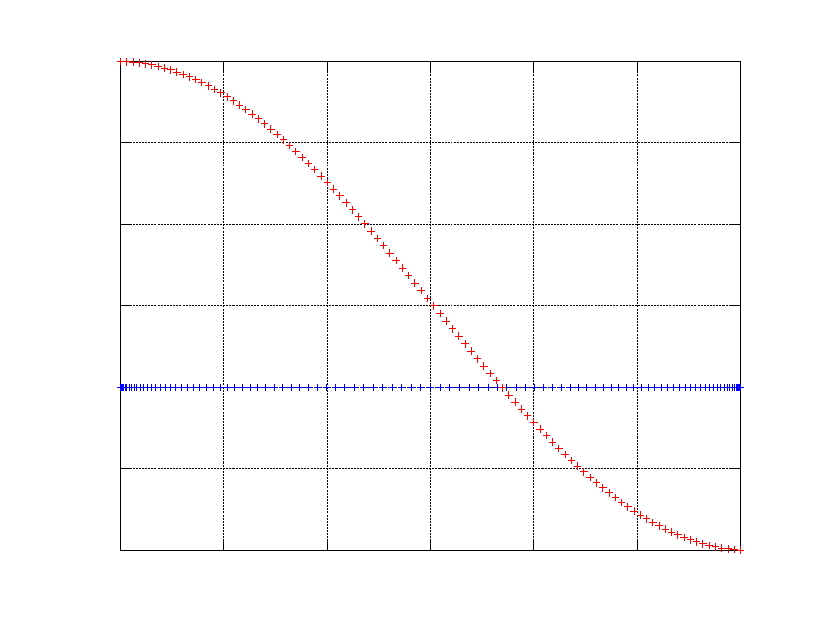
\includegraphics{ApprossimazioneFunzioni/ChecyshevAscissePlotOutput}}%
    \gplfronttext
  \end{picture}%
\endgroup

\end{center}
\begin{center}   
% GNUPLOT: LaTeX picture with Postscript
\begingroup
  \makeatletter
  \providecommand\color[2][]{%
    \GenericError{(gnuplot) \space\space\space\@spaces}{%
      Package color not loaded in conjunction with
      terminal option `colourtext'%
    }{See the gnuplot documentation for explanation.%
    }{Either use 'blacktext' in gnuplot or load the package
      color.sty in LaTeX.}%
    \renewcommand\color[2][]{}%
  }%
  \providecommand\includegraphics[2][]{%
    \GenericError{(gnuplot) \space\space\space\@spaces}{%
      Package graphicx or graphics not loaded%
    }{See the gnuplot documentation for explanation.%
    }{The gnuplot epslatex terminal needs graphicx.sty or graphics.sty.}%
    \renewcommand\includegraphics[2][]{}%
  }%
  \providecommand\rotatebox[2]{#2}%
  \@ifundefined{ifGPcolor}{%
    \newif\ifGPcolor
    \GPcolortrue
  }{}%
  \@ifundefined{ifGPblacktext}{%
    \newif\ifGPblacktext
    \GPblacktexttrue
  }{}%
  % define a \g@addto@macro without @ in the name:
  \let\gplgaddtomacro\g@addto@macro
  % define empty templates for all commands taking text:
  \gdef\gplbacktext{}%
  \gdef\gplfronttext{}%
  \makeatother
  \ifGPblacktext
    % no textcolor at all
    \def\colorrgb#1{}%
    \def\colorgray#1{}%
  \else
    % gray or color?
    \ifGPcolor
      \def\colorrgb#1{\color[rgb]{#1}}%
      \def\colorgray#1{\color[gray]{#1}}%
      \expandafter\def\csname LTw\endcsname{\color{white}}%
      \expandafter\def\csname LTb\endcsname{\color{black}}%
      \expandafter\def\csname LTa\endcsname{\color{black}}%
      \expandafter\def\csname LT0\endcsname{\color[rgb]{1,0,0}}%
      \expandafter\def\csname LT1\endcsname{\color[rgb]{0,1,0}}%
      \expandafter\def\csname LT2\endcsname{\color[rgb]{0,0,1}}%
      \expandafter\def\csname LT3\endcsname{\color[rgb]{1,0,1}}%
      \expandafter\def\csname LT4\endcsname{\color[rgb]{0,1,1}}%
      \expandafter\def\csname LT5\endcsname{\color[rgb]{1,1,0}}%
      \expandafter\def\csname LT6\endcsname{\color[rgb]{0,0,0}}%
      \expandafter\def\csname LT7\endcsname{\color[rgb]{1,0.3,0}}%
      \expandafter\def\csname LT8\endcsname{\color[rgb]{0.5,0.5,0.5}}%
    \else
      % gray
      \def\colorrgb#1{\color{black}}%
      \def\colorgray#1{\color[gray]{#1}}%
      \expandafter\def\csname LTw\endcsname{\color{white}}%
      \expandafter\def\csname LTb\endcsname{\color{black}}%
      \expandafter\def\csname LTa\endcsname{\color{black}}%
      \expandafter\def\csname LT0\endcsname{\color{black}}%
      \expandafter\def\csname LT1\endcsname{\color{black}}%
      \expandafter\def\csname LT2\endcsname{\color{black}}%
      \expandafter\def\csname LT3\endcsname{\color{black}}%
      \expandafter\def\csname LT4\endcsname{\color{black}}%
      \expandafter\def\csname LT5\endcsname{\color{black}}%
      \expandafter\def\csname LT6\endcsname{\color{black}}%
      \expandafter\def\csname LT7\endcsname{\color{black}}%
      \expandafter\def\csname LT8\endcsname{\color{black}}%
    \fi
  \fi
  \setlength{\unitlength}{0.0500bp}%
  \begin{picture}(7680.00,5760.00)%
    \gplgaddtomacro\gplbacktext{%
      \colorrgb{0.00,0.00,0.00}%
      \put(866,633){\makebox(0,0)[r]{\strut{}-1}}%
      \colorrgb{0.00,0.00,0.00}%
      \put(866,1807){\makebox(0,0)[r]{\strut{}-0.5}}%
      \colorrgb{0.00,0.00,0.00}%
      \put(866,2980){\makebox(0,0)[r]{\strut{}0}}%
      \colorrgb{0.00,0.00,0.00}%
      \put(866,4154){\makebox(0,0)[r]{\strut{}0.5}}%
      \colorrgb{0.00,0.00,0.00}%
      \put(866,5327){\makebox(0,0)[r]{\strut{}1}}%
      \colorrgb{0.00,0.00,0.00}%
      \put(998,413){\makebox(0,0){\strut{}-1}}%
      \colorrgb{0.00,0.00,0.00}%
      \put(2486,413){\makebox(0,0){\strut{}-0.5}}%
      \colorrgb{0.00,0.00,0.00}%
      \put(3974,413){\makebox(0,0){\strut{}0}}%
      \colorrgb{0.00,0.00,0.00}%
      \put(5461,413){\makebox(0,0){\strut{}0.5}}%
      \colorrgb{0.00,0.00,0.00}%
      \put(6949,413){\makebox(0,0){\strut{}1}}%
    }%
    \gplgaddtomacro\gplfronttext{%
    }%
    \gplbacktext
    \put(0,0){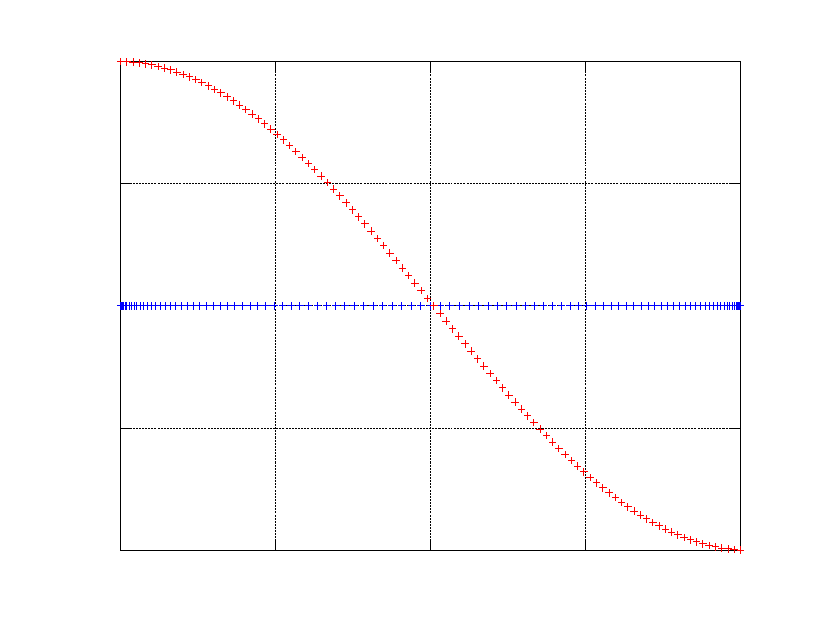
\includegraphics{ApprossimazioneFunzioni/ChecyshevAscisseUnaryPlotOutput}}%
    \gplfronttext
  \end{picture}%
\endgroup

\end{center}

\begin{exercise}[4.15]
Per il testo dell'esercizio consultare il libro di testo.
\end{exercise}
Per il codice che implementa le richieste dell'esercizio e produce i seguenti
risultati vedere \nameref{subsec:exercise415}.

Nei seguenti grafici in
\emph{rosso} \`e rappresentata la funzione di \emph{Bernstein}, mentre in 
\emph{blu} \`e rappresentata la funzione di \emph{Runge}. Questo primo grafico
ha l'asse delle ordinate costruito in modo logaritmico:
\begin{center}   
% GNUPLOT: LaTeX picture with Postscript
\begingroup
  \makeatletter
  \providecommand\color[2][]{%
    \GenericError{(gnuplot) \space\space\space\@spaces}{%
      Package color not loaded in conjunction with
      terminal option `colourtext'%
    }{See the gnuplot documentation for explanation.%
    }{Either use 'blacktext' in gnuplot or load the package
      color.sty in LaTeX.}%
    \renewcommand\color[2][]{}%
  }%
  \providecommand\includegraphics[2][]{%
    \GenericError{(gnuplot) \space\space\space\@spaces}{%
      Package graphicx or graphics not loaded%
    }{See the gnuplot documentation for explanation.%
    }{The gnuplot epslatex terminal needs graphicx.sty or graphics.sty.}%
    \renewcommand\includegraphics[2][]{}%
  }%
  \providecommand\rotatebox[2]{#2}%
  \@ifundefined{ifGPcolor}{%
    \newif\ifGPcolor
    \GPcolortrue
  }{}%
  \@ifundefined{ifGPblacktext}{%
    \newif\ifGPblacktext
    \GPblacktexttrue
  }{}%
  % define a \g@addto@macro without @ in the name:
  \let\gplgaddtomacro\g@addto@macro
  % define empty templates for all commands taking text:
  \gdef\gplbacktext{}%
  \gdef\gplfronttext{}%
  \makeatother
  \ifGPblacktext
    % no textcolor at all
    \def\colorrgb#1{}%
    \def\colorgray#1{}%
  \else
    % gray or color?
    \ifGPcolor
      \def\colorrgb#1{\color[rgb]{#1}}%
      \def\colorgray#1{\color[gray]{#1}}%
      \expandafter\def\csname LTw\endcsname{\color{white}}%
      \expandafter\def\csname LTb\endcsname{\color{black}}%
      \expandafter\def\csname LTa\endcsname{\color{black}}%
      \expandafter\def\csname LT0\endcsname{\color[rgb]{1,0,0}}%
      \expandafter\def\csname LT1\endcsname{\color[rgb]{0,1,0}}%
      \expandafter\def\csname LT2\endcsname{\color[rgb]{0,0,1}}%
      \expandafter\def\csname LT3\endcsname{\color[rgb]{1,0,1}}%
      \expandafter\def\csname LT4\endcsname{\color[rgb]{0,1,1}}%
      \expandafter\def\csname LT5\endcsname{\color[rgb]{1,1,0}}%
      \expandafter\def\csname LT6\endcsname{\color[rgb]{0,0,0}}%
      \expandafter\def\csname LT7\endcsname{\color[rgb]{1,0.3,0}}%
      \expandafter\def\csname LT8\endcsname{\color[rgb]{0.5,0.5,0.5}}%
    \else
      % gray
      \def\colorrgb#1{\color{black}}%
      \def\colorgray#1{\color[gray]{#1}}%
      \expandafter\def\csname LTw\endcsname{\color{white}}%
      \expandafter\def\csname LTb\endcsname{\color{black}}%
      \expandafter\def\csname LTa\endcsname{\color{black}}%
      \expandafter\def\csname LT0\endcsname{\color{black}}%
      \expandafter\def\csname LT1\endcsname{\color{black}}%
      \expandafter\def\csname LT2\endcsname{\color{black}}%
      \expandafter\def\csname LT3\endcsname{\color{black}}%
      \expandafter\def\csname LT4\endcsname{\color{black}}%
      \expandafter\def\csname LT5\endcsname{\color{black}}%
      \expandafter\def\csname LT6\endcsname{\color{black}}%
      \expandafter\def\csname LT7\endcsname{\color{black}}%
      \expandafter\def\csname LT8\endcsname{\color{black}}%
    \fi
  \fi
  \setlength{\unitlength}{0.0500bp}%
  \begin{picture}(7680.00,5760.00)%
    \gplgaddtomacro\gplbacktext{%
      \colorrgb{0.00,0.00,0.00}%
      \put(866,633){\makebox(0,0)[r]{\strut{}$10^{-4}$}}%
      \colorrgb{0.00,0.00,0.00}%
      \put(866,1806){\makebox(0,0)[r]{\strut{}$10^{-3}$}}%
      \colorrgb{0.00,0.00,0.00}%
      \put(866,2980){\makebox(0,0)[r]{\strut{}$10^{-2}$}}%
      \colorrgb{0.00,0.00,0.00}%
      \put(866,4154){\makebox(0,0)[r]{\strut{}$10^{-1}$}}%
      \colorrgb{0.00,0.00,0.00}%
      \put(866,5327){\makebox(0,0)[r]{\strut{}$10^{0}$}}%
      \colorrgb{0.00,0.00,0.00}%
      \put(998,413){\makebox(0,0){\strut{}0}}%
      \colorrgb{0.00,0.00,0.00}%
      \put(2188,413){\makebox(0,0){\strut{}5}}%
      \colorrgb{0.00,0.00,0.00}%
      \put(3378,413){\makebox(0,0){\strut{}10}}%
      \colorrgb{0.00,0.00,0.00}%
      \put(4569,413){\makebox(0,0){\strut{}15}}%
      \colorrgb{0.00,0.00,0.00}%
      \put(5759,413){\makebox(0,0){\strut{}20}}%
      \colorrgb{0.00,0.00,0.00}%
      \put(6949,413){\makebox(0,0){\strut{}25}}%
    }%
    \gplgaddtomacro\gplfronttext{%
    }%
    \gplbacktext
    \put(0,0){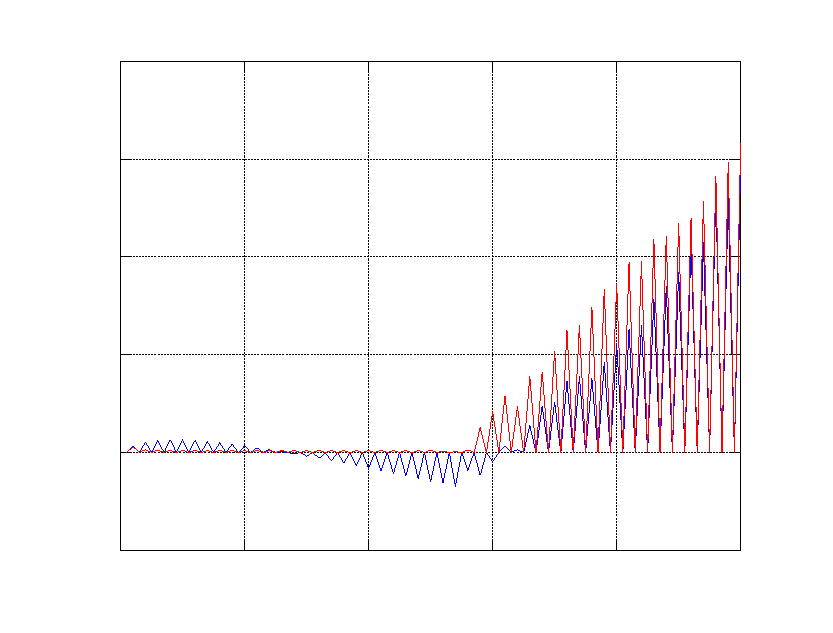
\includegraphics{ApprossimazioneFunzioni/exercise415-ErrorsSemilogYPlotOutput}}%
    \gplfronttext
  \end{picture}%
\endgroup

\end{center}
Riporto lo stesso dataset di errori per le due curve, costruendo entrambi gli
assi in modo logaritmico:
\begin{center}  
% GNUPLOT: LaTeX picture with Postscript
\begingroup
  \makeatletter
  \providecommand\color[2][]{%
    \GenericError{(gnuplot) \space\space\space\@spaces}{%
      Package color not loaded in conjunction with
      terminal option `colourtext'%
    }{See the gnuplot documentation for explanation.%
    }{Either use 'blacktext' in gnuplot or load the package
      color.sty in LaTeX.}%
    \renewcommand\color[2][]{}%
  }%
  \providecommand\includegraphics[2][]{%
    \GenericError{(gnuplot) \space\space\space\@spaces}{%
      Package graphicx or graphics not loaded%
    }{See the gnuplot documentation for explanation.%
    }{The gnuplot epslatex terminal needs graphicx.sty or graphics.sty.}%
    \renewcommand\includegraphics[2][]{}%
  }%
  \providecommand\rotatebox[2]{#2}%
  \@ifundefined{ifGPcolor}{%
    \newif\ifGPcolor
    \GPcolortrue
  }{}%
  \@ifundefined{ifGPblacktext}{%
    \newif\ifGPblacktext
    \GPblacktexttrue
  }{}%
  % define a \g@addto@macro without @ in the name:
  \let\gplgaddtomacro\g@addto@macro
  % define empty templates for all commands taking text:
  \gdef\gplbacktext{}%
  \gdef\gplfronttext{}%
  \makeatother
  \ifGPblacktext
    % no textcolor at all
    \def\colorrgb#1{}%
    \def\colorgray#1{}%
  \else
    % gray or color?
    \ifGPcolor
      \def\colorrgb#1{\color[rgb]{#1}}%
      \def\colorgray#1{\color[gray]{#1}}%
      \expandafter\def\csname LTw\endcsname{\color{white}}%
      \expandafter\def\csname LTb\endcsname{\color{black}}%
      \expandafter\def\csname LTa\endcsname{\color{black}}%
      \expandafter\def\csname LT0\endcsname{\color[rgb]{1,0,0}}%
      \expandafter\def\csname LT1\endcsname{\color[rgb]{0,1,0}}%
      \expandafter\def\csname LT2\endcsname{\color[rgb]{0,0,1}}%
      \expandafter\def\csname LT3\endcsname{\color[rgb]{1,0,1}}%
      \expandafter\def\csname LT4\endcsname{\color[rgb]{0,1,1}}%
      \expandafter\def\csname LT5\endcsname{\color[rgb]{1,1,0}}%
      \expandafter\def\csname LT6\endcsname{\color[rgb]{0,0,0}}%
      \expandafter\def\csname LT7\endcsname{\color[rgb]{1,0.3,0}}%
      \expandafter\def\csname LT8\endcsname{\color[rgb]{0.5,0.5,0.5}}%
    \else
      % gray
      \def\colorrgb#1{\color{black}}%
      \def\colorgray#1{\color[gray]{#1}}%
      \expandafter\def\csname LTw\endcsname{\color{white}}%
      \expandafter\def\csname LTb\endcsname{\color{black}}%
      \expandafter\def\csname LTa\endcsname{\color{black}}%
      \expandafter\def\csname LT0\endcsname{\color{black}}%
      \expandafter\def\csname LT1\endcsname{\color{black}}%
      \expandafter\def\csname LT2\endcsname{\color{black}}%
      \expandafter\def\csname LT3\endcsname{\color{black}}%
      \expandafter\def\csname LT4\endcsname{\color{black}}%
      \expandafter\def\csname LT5\endcsname{\color{black}}%
      \expandafter\def\csname LT6\endcsname{\color{black}}%
      \expandafter\def\csname LT7\endcsname{\color{black}}%
      \expandafter\def\csname LT8\endcsname{\color{black}}%
    \fi
  \fi
  \setlength{\unitlength}{0.0500bp}%
  \begin{picture}(7680.00,5760.00)%
    \gplgaddtomacro\gplbacktext{%
      \colorrgb{0.00,0.00,0.00}%
      \put(866,634){\makebox(0,0)[r]{\strut{}$10^{-5}$}}%
      \colorrgb{0.00,0.00,0.00}%
      \put(866,1573){\makebox(0,0)[r]{\strut{}$10^{0}$}}%
      \colorrgb{0.00,0.00,0.00}%
      \put(866,2511){\makebox(0,0)[r]{\strut{}$10^{5}$}}%
      \colorrgb{0.00,0.00,0.00}%
      \put(866,3450){\makebox(0,0)[r]{\strut{}$10^{10}$}}%
      \colorrgb{0.00,0.00,0.00}%
      \put(866,4388){\makebox(0,0)[r]{\strut{}$10^{15}$}}%
      \colorrgb{0.00,0.00,0.00}%
      \put(866,5327){\makebox(0,0)[r]{\strut{}$10^{20}$}}%
      \colorrgb{0.00,0.00,0.00}%
      \put(998,414){\makebox(0,0){\strut{}$10^{0}$}}%
      \colorrgb{0.00,0.00,0.00}%
      \put(3974,414){\makebox(0,0){\strut{}$10^{1}$}}%
      \colorrgb{0.00,0.00,0.00}%
      \put(6950,414){\makebox(0,0){\strut{}$10^{2}$}}%
    }%
    \gplgaddtomacro\gplfronttext{%
    }%
    \gplbacktext
    \put(0,0){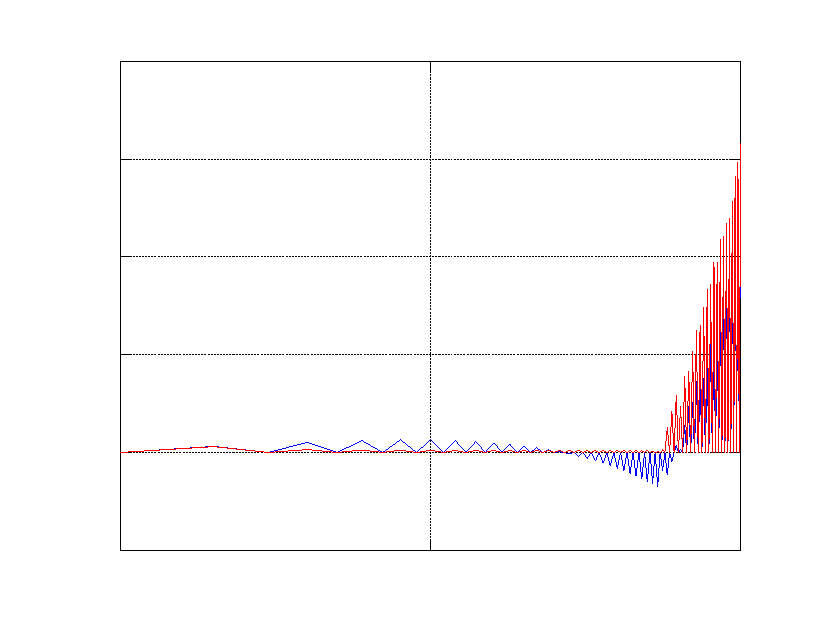
\includegraphics{ApprossimazioneFunzioni/exercise415-ErrorsLoglogPlotOutput}}%
    \gplfronttext
  \end{picture}%
\endgroup

\end{center}
Per entrambi i grafici, le valutazioni della rispettiva funzione, del polinomio
interpolante e la costruzione del polinomio interpolante sono riferiti ai
rispettivi dominii $[a,b]$ definiti nel testo dell'esercizio. 

Possiamo notare che l'errore diverge all'aumentare del numero di ascisse di
interpolazione, ma con un rate molto pi\`u basso rispetto ai plot riportati
nell'esercizio \ref{exercise:exercise411}. Inoltre si vede che la curva
che modella l'errore effettua un effetto ``jo-jo'' al crescere di $n$.
